\section{Approximation Algorithms}

\begin{frame}
  \frametitle{Why should we look for an approximation?}
  \begin{block}{Static graphs}
    \begin{itemize}
      \item many interesting networks are \emph{web-scale};
      \item computing the exact centralities can be extremely expensive;
      \item is there a real reason (i.e., application) to \emph{require} the
        exact values?
    \end{itemize}
  \end{block}
  \pause
  \begin{block}{Dynamic graphs}
    \begin{itemize}
      \item exact centralities change at all times;
      \item not worth chasing for highly volatile quantities;
    \end{itemize}
  \end{block}
  \pause
  In both cases, \emph{high quality} approximations are \emph{sufficient in
  practice}
\end{frame}

\begin{frame}
  \frametitle{What kind of approximation}
  \begin{itemize}
    \item $v$: vertex with exact centrality $c(v)$
    \item $\tilde{c}(v)$: value that ``approximates'' $c(v)$
  \end{itemize}
  \begin{definition}[Absolute error]
    \centering
    $\mathsf{err}_\mathrm{abs}(v)=|c(v)-\tilde{c}(v)|$
  \end{definition}
  \begin{definition}[Relative error]
    \centering
    $\mathsf{err}_\mathrm{rel}(v)=|c(v)-\tilde{c}(v)|/c(v)$
  \end{definition}
  \pause
  \begin{definition}[$(\varepsilon,\delta)$-approximation]
    \begin{itemize}
      \item Let $\varepsilon\in(0,1)$ and $\delta\in(0,1)$;
      \item a \emph{$(\varepsilon,\delta)$-approximation} is a \emph{set}
        $\{\tilde{c}(v), v\in V\}$ of $n$ values, such that
        \[
          \Pr\left(\exists v\in V \text{ s.t. } \mathsf{err}(v)
          >\varepsilon\right)\le \delta;
        \]
        \vspace{-20pt}
      \pause
      \item it offers \emph{uniform probabilistic guarantees} over all the
        nodes;
        \pause
      \item it assumes \emph{normalized} versions of centrality (i.e., in
        $[0,1]$).
    \end{itemize}
  \end{definition}
\end{frame}

\begin{frame}
  \frametitle{Sampling}
  Many of the algorithms we present are \emph{sampling-based}.
  \begin{block}{General Sampling Based Algorithm}
    \begin{enumerate}
      \item Select \emph{independently at random} (not all \emph{uniformly})
        a \emph{small} set of \emph{objects} (e.g., single vertices, pair of vertices, shortest
        paths);
        \pause
      \item Perform some computation using these objects (e.g., SSSP from vertex);
        \pause
      \item Use the results of the computation to estimate the centrality of all
        nodes;
    \end{enumerate}
  \end{block}
\end{frame}

\begin{frame}
  \frametitle{Sampling}
  \begin{block}{Why sampling?}
    By only select a small subset of the ``objects'' (instead of the whole set),
    computing the approximation is faster than computing the exact values
  \end{block}
  \pause
  \begin{block}{Questions for sampling algorithms}
    \begin{itemize}
      \item What ``objects'' to sample?
        \pause
      \item How to sample?\\
        \quad If sampling procedure is slow, then the advantages are lost;
        \pause
      \item How many objects to sample in order to guarantee an
        $(\varepsilon,\delta)$-approximation?
    \end{itemize}
  \end{block}
\end{frame}

\begin{frame}
  \frametitle{Outline}
  \begin{itemize}
    \item Approximation algorithms for static graphs
      \begin{itemize}
        \item A sampling-based algorithm for closeness
        \item A sampling+pivoting algorithm for closeness
        \item Two sampling-based algorithms for betweenness
      \end{itemize}
    \item Approximation algorithms for dynamic graphs
      \begin{itemize}
        \item Two sampling-based algorithms for betweenness
      \end{itemize}
  \end{itemize}
\end{frame}

\subsection{Approximation Algorithms for Static Graphs}

\begin{frame}
  \centering
  \vfill
  {\huge Fast approximation of centrality}
  \vfill
  {\Large D.~Eppstein, J.~Wang}
  \vfill
  {\large Journal of Graph Algorithms and Applications (2004)}
  \vfill
\end{frame}

\begin{frame}
  \frametitle{Idea}
  \vfill
  Interested in approximating \emph{closeness}:
  \[
    \closeness(x)=\frac{n-1}{\sum_{y\neq x}d(x,y)}
  \]
  (inverse of the average distance)
  \vfill
  Fastest-known exact algorithm: APSP\\
  \qquad I.e., run Dijkstra's algorithm from \emph{each} vertex $v$
  \pause
  \vfill
  Idea: only run Dijkstra from \emph{a few sources}!
  \vfill
  \pause
  \begin{block}{Warning}
    The algorithm actually computes an approximation for
    the \emph{inverse} of closeness:
    \[
      \closeness^{-1}(v)=\frac{\sum_{y\neq x}d(u,v)}{n-1}
    \]
    (effectively the average distance)
  \end{block}
\end{frame}

\begin{frame}
  \frametitle{Algorithm}
  \begin{block}{}
    \begin{itemize}
      \item Let $k$ be the number of sources to obtain the desired
        approximation;
        \pause
      \item For $i=1,\dotsc, k$:
        \begin{itemize}
          \item pick a vertex $u_i$ uniformly at random
            \pause
          \item run Dijkstra from $u_i$
        \end{itemize}
      \item Let
        \[
          \widetilde{\closeness^{-1}}(v)=\frac{n}{n-1}\frac{\sum_{i=1}^k
          d(u_i,v_i)}{k}
        \]
    \end{itemize}
  \end{block}
  \pause
  \begin{theorem}
    $\mathbb{E}\left[\widetilde{\closeness^{-1}}(v)\right]=\closeness^{-1}(v)$.
  \end{theorem}
  \pause
  \begin{block}{Question}
    How large should $k$ be to get a good approximation of $\closeness^{-1}$?
  \end{block}
\end{frame}

%\begin{frame}
%  \frametitle{Hoeffding Inequality}
%  \begin{itemize}
%    \item A concentration inequality for the sum of independent random
%      variables;
%    \item It allows to study the trade-off between the error (difference between
%      sample value and expectation) and the sample size;
%  \end{itemize}
%  \pause
%  \begin{theorem}[Hoeffding Inequality]
%    Let $x_1,\dotsc, x_n$ be independent r.v., with
%    \begin{itemize}
%      \item $a_i\le x_i\le b_i$
%      \item $\mu=\mathbb{E}[\sum x_i/k]$
%    \end{itemize}
%    Then, for $\xi > 0$,
%    \[
%      \Pr\left(\left|\frac{\sum_{i=1}^kx_i}{k}-\mu\right|\ge\xi\right)\le
%      2e^{-2k^2\xi^2/\sum_{i=1}^k(b_i-a_i)^2}
%    \]
%  \end{theorem}
%\end{frame}

\begin{frame}
  \frametitle{How much to sample}
  \begin{lemma}
    Let $\Delta$ be the diameter of the graph and let
    $\varepsilon,\delta\in(0,1)$. If
    \[
      k\ge\frac{2}{\varepsilon^2} \left(\ln 2 + \ln n +
      \ln\frac{1}{\delta}\right)
    \]
    Then, with probability at least $1-\delta$
    \[
      \left|\widetilde{\closeness^{-1}}(v)-\closeness^{-1}(v)\right| \le
      \Delta\varepsilon, \text{ for all } v\in V
    \]
  \end{lemma}
  \pause
  \begin{block}{Proof}
    \begin{enumerate}
      \item \emph{Hoeffding inequality} to bound the error of a single vertex;
      \item \emph{Union bound} to get uniform guarantees.
    \end{enumerate}
  \end{block}
  \pause
  Running time: $O\left(\frac{\log n - \log \delta}{\varepsilon^2}(n\log n +
  m)\right)$.
\end{frame}

\begin{frame}
  \centering
  \vfill
  {\huge Computing Classic Closeness Centrality, at Scale}
  \vfill
  {\Large E.~Cohen, D.~Delling, T.~Pajor, R.~F.~Werneck}
  \vfill
  {\large COSN '14: ACM Conference on Social Networks (2014) }
  \vfill
\end{frame}

\begin{frame}
  \frametitle{Issues with sampling}
  \begin{itemize}
    \item Assume that the distance distribution from a vertex $v$ has a
      \emph{heavy tail}, then the average distance
      \[
        \closeness^{-1}(v)=\frac{\sum_{u\neq v}d(u,v)}{n-1}\enspace
      \]
      is dominated by few distant vertices;
    \pause
    \item it is unlikely that these vertices are among the $k$ that are sampled
    \item Hence the sample average
      \[
        \widetilde{\closeness^{-1}}(v)=\frac{n}{n-1}\frac{\sum_{i=1}^k
        d(u_i,v_i)}{k}
      \]
      is a \emph{poor estimator} of the average distance $\closeness^{-1}(v)$.
    \pause
    \item Sampling along can't give us \emph{small relative error}
  \end{itemize}
\end{frame}

\begin{frame}
  \frametitle{Pivoting}
  \begin{definition}{Pivot}
    The \emph{pivot} $p(v)$ of a vertex $v$ is the sampled vertex which is
    closest to $v$ ($p(v)\in\Sam$).
  \end{definition}
  \begin{itemize}
    \item We have the exact value of $\closeness^{-1}(p(v))$, can we leverage
      it?
    \pause
    \item The average SP distance $\closeness^{-1}(v)$ of $v$ is ``close'' to
      $\closeness^{-1}(p(v))$:
      \[
        \closeness^{-1}(p(v))-d(v,p(v)) \le \closeness^{-1}(c) \le \closeness^{-1}(p(v))-d(v,p(v))
      \]
    \vspace{-20pt}
    \pause
    \item One can actually prove that, with high probability,
      \[
        \closeness^{-1}(p(v))+d(v,p(v))\le 3\closeness^{-1}(v)+O(1)
      \]
      \vspace{-20pt}
  \end{itemize}
  \pause
  Pivoting by itself is not satisfactory: the relative error is still somewhat
  large.
  \vfill
  \pause
  Idea: \emph{combine sampling and pivoting} into a hybrid estimator
\end{frame}

\begin{frame}
  \frametitle{Hybrid Estimator}
  For each vertex $v$ with pivot $p(v)$, split the set $V\setminus\Sam$ into
  three sets:
  \pause
  \begin{itemize}
    \item $L(v)$: vertices in $V\setminus\Sam$ at distance at most $d(v,p(v))$
      from $p(v)$;
    \pause
    \item $HC(v)$: vertices in $\Sam$ with distance greater than $d(v,p(v))$
      from $p(v)$.
    \pause
    \item $H(v)$: vertices in $V\setminus\Sam$ at distance greater than
      $d(v,p(v))$ from $p(v)$.
  \end{itemize}
  \pause
  The hybrid estimator is
  \begin{align*}
    \widetilde{\closeness^{-1}}(v)=&\frac{1}{n-1}\sum_{u\in
    H(v)}d(p(v),u)+\sum_{u\in HC(v)}d(u,v)\\
    &+\frac{|L(v)|}{|L(v)\cap\Sam|}\sum_{u\in L(v)\cap\Sam}d(u,v)
  \end{align*}
  \pause
  We have $\mathbb{E}[\widetilde{\closeness^{-1}}(v)]\neq\closeness^{-1}(v)$.
\end{frame}

\begin{frame}
  \frametitle{Guarantees}
  \begin{theorem}
    \begin{itemize}
      \item With $k=1/\varepsilon^3$, the hybrid estimator has \emph{normalized
        RMSE} $O(\varepsilon)$.
      \item With $k=\varepsilon^{-1}\ln n$, the maximum relative error is
        $O(\varepsilon)$ w.h.p.
    \end{itemize}
  \end{theorem}
\end{frame}

\begin{frame}
  \frametitle{Experiments}
  \begin{figure}
    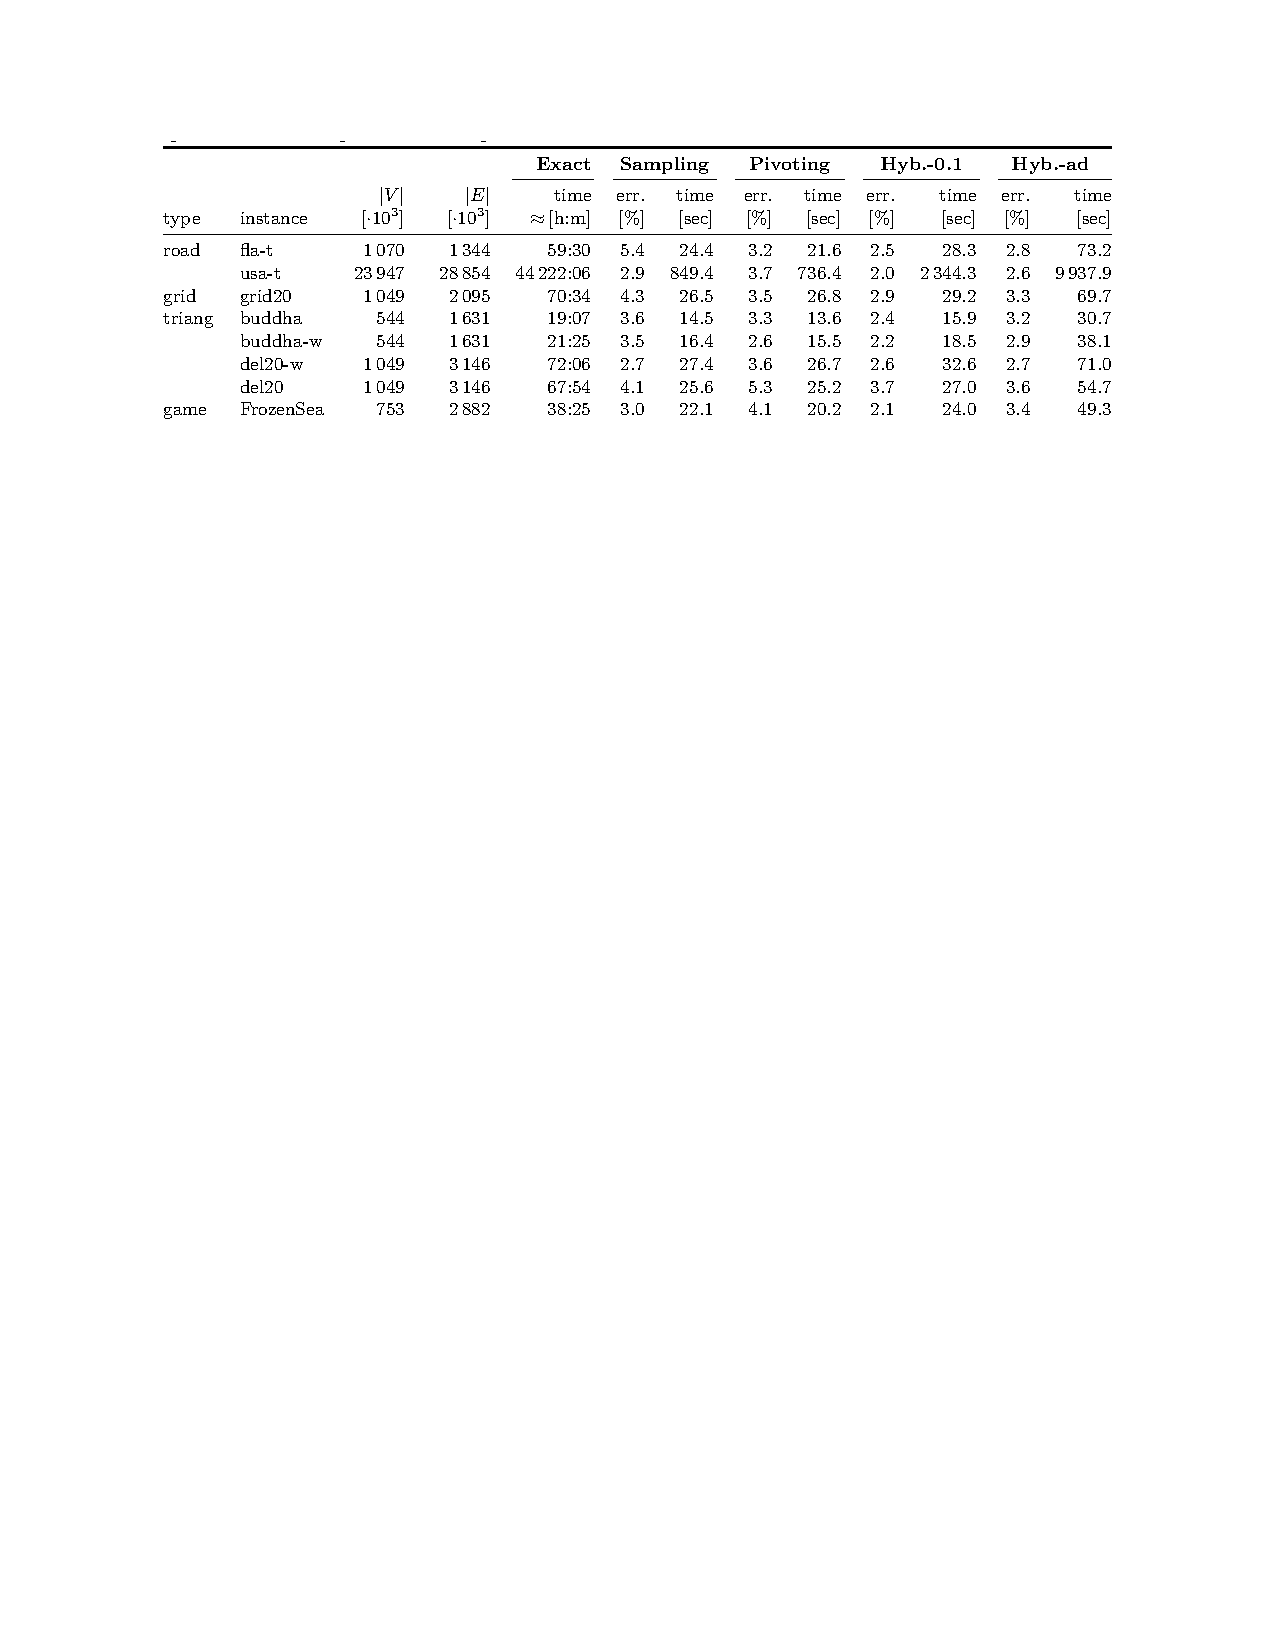
\includegraphics[width=\textwidth]{imgs/cohenhybrid.pdf}
  \end{figure}
  The hybrid estimator is better than just-sampling and just-pivoting.
\end{frame}

\begin{frame}
  \frametitle{Summary for closeness}
  \begin{itemize}
    \item Sampling can help, but not alone
    \item Pivoting alone is not good
    \item The hybrid approach is promising, but the sample size results are
      somewhat disappointing (very large sample sizes!)
  \end{itemize}
  More work to do!
\end{frame}

\begin{frame}
  \centering
  \vfill
  {\Huge Centrality Estimation in Large Networks}
  \vfill
  {\Large U.~Brandes, C.~Pich}
  \vfill
  {\large International Journal of Bifurcation and Chaos (2007)}
  \vfill
\end{frame}

\begin{frame}
  \frametitle{Betweenness centrality}
  We consider a \emph{normalized} version:
  \[
    \betw(v)=\frac{1}{n(n-1)}\sum_{s,t\neq v}\frac{\sigma_{st}(v)}{\sigma_{st}}\in[0,1]
  \]
  \begin{itemize}
    \item $\sigma_{st}$: number of SPs from $s$ to $t$
    \item $\sigma_{st}(v)$: number of SPs from $s$ to $t$ going through $v$
  \end{itemize}
  \pause
  Exact algorithm: Brandes' Algorithm
  \begin{enumerate}
    \item Run Dijkstra's algorithm \emph{from each source vertex $s$}
    \item After each run, perform aggregation by walking SP DAG backwards
  \end{enumerate}
  \pause
  Idea: run Dijkstra only from a few sources (as in EW'01)
\end{frame}

\begin{frame}
  \frametitle{How can one get an $(\varepsilon,\delta)$-approximation?}
  \begin{algorithm}[H]
    \DontPrintSemicolon
    $k\leftarrow \frac{1}{\varepsilon^2}\left(\ln n + \ln 2 +
    \ln\frac{1}{\delta}\right)$ \texttt{// sample size}\;
    $\tilde{\betw}(v)\leftarrow 0$, for all $v\in V$\;
    \For(\texttt{// Brandes' algo iterates over $V$}){$i\leftarrow 1,\dotsc,k$} {
      $v_i \leftarrow$ random vertex from $V$, chosen uniformly\;
      Perform single-source SP computation from $v_i$\;
      Perform partial aggregation, updating $\tilde{\betw}(u)$, $u\in V$,
      like in exact algorithm\;
    }
    Output $\{\tilde{\betw(v)}, v\in V\}$\;
  \end{algorithm}
  \vfill
  \pause
  \begin{theorem}
    The output is a $(\varepsilon,\delta)$-approximation:
    \[
      \Pr\left(\exists v\in V \text{ s.t. }
      |\tilde{\betw}(v)-\betw{v}|>\varepsilon\right)\le \delta
    \]
  \end{theorem}
\end{frame}

\begin{frame}
  \frametitle{How do they prove it?}
  Start with bounding the deviation for a single vertex $v$ (Hoeffding inequality):
  \[
    \Pr(|\tilde{\betw}(v)-\betw(v)|>\varepsilon)\le 2e^{-2k\varepsilon^2}
  \]
  \vfill
  Then take the union bound over $n$ vertices to ensure uniform convergence
  \vfill
  The sample size $k$ must be such that
  \[
    2e^{-2k\varepsilon^2}\le\frac{\delta}{n}
  \]
  That is, to get an $(\varepsilon,\delta)$-approximation, we need
  \[
    k\ge\frac{1}{2\varepsilon^2}\left(\ln n + \ln 2 +
    \ln\frac{1}{\delta}\right)
  \]
\end{frame}

\begin{frame}
  \centering
  \vfill
  {\huge Better Approximation of Betweenness Centrality}
  \vfill
  {\Large R.~Geisberger, P.~Sanders, D.~Schultes}
  \vfill
  {\large ALENEX (2008)}
  \vfill
\end{frame}

\begin{frame}
  \frametitle{Issues with standard estimator}
    The standard estimator
    \[
      \tbetw(v)=\frac{1}{k}\sum_{i=1}^k \delta_{u_i}(v)
    \]
    produces large overestimates for unimportant vertices close to a sampled
    vertex
  \pause
  \begin{block}{Example}
    \begin{itemize}
      \item Let $v$ be a degree-two vertex connecting a degree-one vertex $u$ to
        the rest of the network;
      \item If $u$ is sampled, then $\tbetw(v)$ overestimates $\betw(v)$ by a
        factor of $n/k$
    \end{itemize}
  \end{block}
  \pause
  Possible solution: stop vertices from ``profiting'' for being near a sampled
  vertex.
\end{frame}

\begin{frame}
  \frametitle{A new sampling scheme}
  Idea: sample \emph{pairs} $(s,d)$ of vertex and \emph{direction} (`forward'' or
  ``backward'')
  \pause
  \begin{itemize}
    \item When sampling $(s,\text{forward})$
      \begin{itemize}
        \item run Dijkstra from $s$
      \end{itemize}
      \pause
    \item When sampling $(t,\text{backward}$)
      \begin{itemize}
        \item virtually flip direction of edges (if directed graph);
        \item run Dijkstra from $s$
      \end{itemize}
  \end{itemize}
  \pause
  We need to adapt the estimator $\tbetw(v)$.
\end{frame}

\begin{frame}
  \frametitle{New estimator}
  For a vertex $v$, define
  \[
    g_v(u,d)=\left\{\begin{array}{ll}
        \sum_{t\in V,t\neq u,v} \frac{\sigma_{ut}(v)}{\sigma_{ut}}\frac{d(u,v)}{d(v,t)}
        & \text{if } d=\text{forward}\\
        \sum_{t\in V,t\neq u,v}
        \frac{\sigma_{ut}(v)}{\sigma_{ut}}\left(1-\frac{d(u,v)}{d(v,t)}\right)
        & \text{if } d=\text{backward}\end{array}\right.
  \]
  \pause
  The new estimator for $\betw(v)$ is
  \[
    \tbetw(v)=\frac{2}{k}\sum_{i=1}^k g_v(u_i,d_i)
  \]
  The factor $2$ corrects for the reduced sampling probabilities ($1/2n$)
  \pause
  \begin{theorem}
    If
    \[
      k\ge XXX,
    \]
    then the output is a $(\varepsilon,\delta)$-approximation:
    \[
      \Pr\left(\exists v\in V \text{ s.t. }
      |\tilde{\betw}(v)-\betw{v}|>\varepsilon\right)\le \delta
    \]
    \vspace{-10pt}
  \end{theorem}
\end{frame}

\begin{frame}
  \frametitle{Experiments}
  \begin{figure}
    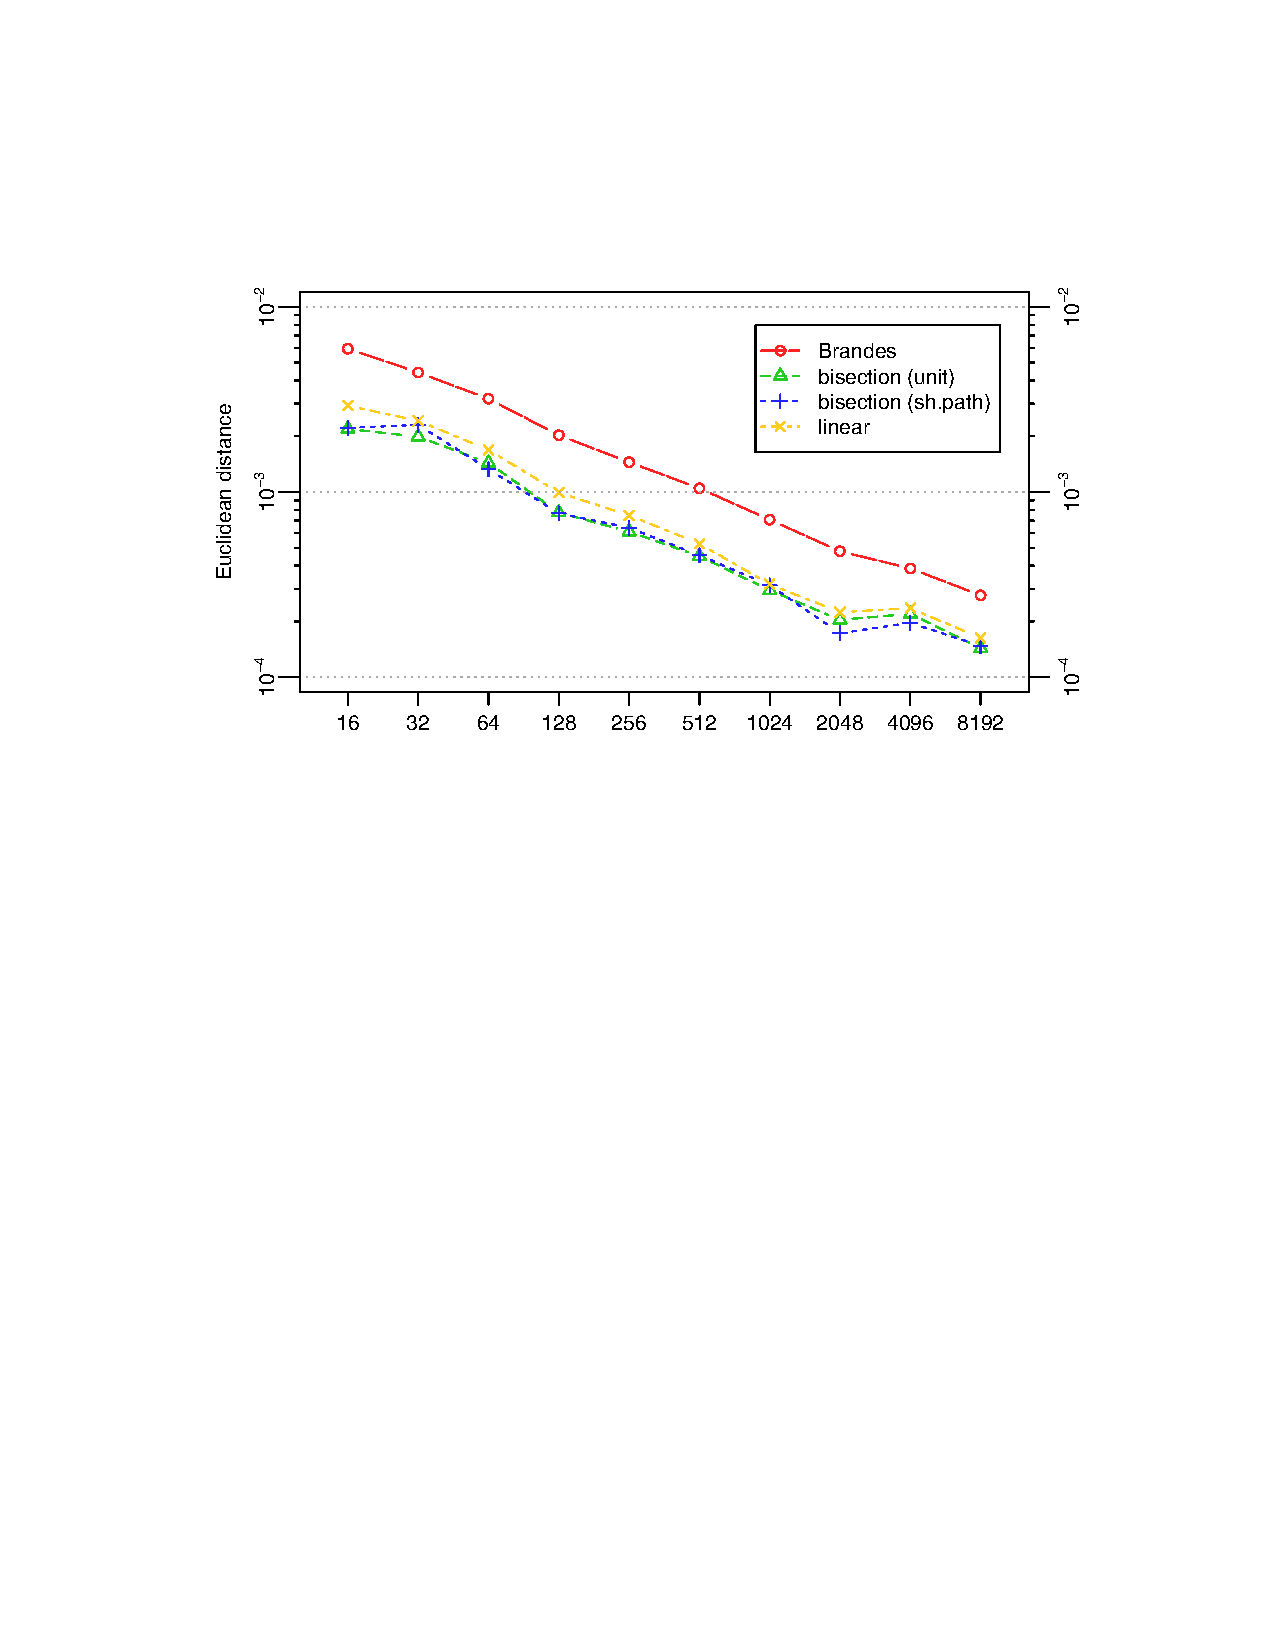
\includegraphics[width=\textwidth]{imgs/geisberger.pdf}
  \end{figure}
  \vspace{-30pt}
  \begin{center}
    Sample size
  \end{center}
  Euclidean distance between the vector of exact centralities and the vector of
  estimated centralities.
\end{frame}

\begin{frame}
  \centering
  \vfill
  {\huge Fast Approximation of Betweenness Centrality through Sampling}
  \vfill
  {\Large M.~Riondato, E.~M.~Kornaropoulos}
  \vfill
  {\large DMKD: Data Mining and Knowledge Discovery (2015)}
  \vfill
\end{frame}

\begin{frame}
  \frametitle{What is wrong with this sampling approach?}
  1) The algorithm needs
  \[
    k\ge\frac{1}{2\varepsilon^2}\left(\ln n + \ln 2 +
    \ln\frac{1}{\delta}\right)
  \]
  \begin{itemize}
    \item This is \emph{loose due to the union bound}, and does not scale well
      (experiments)
    \pause
    \item The sample size depends on $\ln n$. This is \emph{not the right
      quantity}: not all graphs of $n$ nodes are equally ``difficult'': e.g., the $n$-star is ``easier'' than a random graph
  \end{itemize}
  \pause
  The sample size $k$ should depend on a more \emph{specific characteristic
  quantity of the graph}
  \vfill
  \pause
  2) At each iteration, the algorithm performs a SSSP computation\\
  \quad \emph{Full exploration} of the graph, no locality
\end{frame}

\begin{frame}
  \frametitle{How can we improve the sample size?}
  [R. and Kornaropoulos, 2015] present an algorithm that:
  \vfill
  1) uses a sample size which depends on the \emph{vertex-diameter}, a
  characteristic quantity of the graph.\\
  \qquad The derivation uses the \emph{VC-dimension} of the problem;
  \pause
  \vfill
  2) samples SPs according to a specific, \emph{non-uniform distribution} over
  the set $\mathbb{S}_G$ of \emph{all SPs in the graph}. For each sample, it
  performs a single $s-t$ SP computation
  \begin{itemize}
    \item More locality: fewer edges touched than single-source SP
    \item Can use bidirectional search / A\textsuperscript{*},
      \ldots
  \end{itemize}
\end{frame}

\begin{frame}
  \frametitle{What is the algorithm?}
  \begin{algorithm}[H]
    \DontPrintSemicolon
    $\mathsf{VD}(G)\leftarrow$ vertex-diameter of $G$ \texttt{// stay
    tuned!}\;
    $k\leftarrow\frac{1}{2\varepsilon^2}\left(\lfloor\log_2(\mathsf{VD}(G)-2\rfloor)
    +1 + \ln(1/\delta)\right)$ \texttt{// sample size}\;
    $\tilde{\betw}(v)\leftarrow 0$, for all $v\in V$\;
    \For{$i\leftarrow 1\dotsc,k$}{
      $(u,v)\leftarrow$ random pair of different vertices, chosen
      uniformly\;
      $\mathcal{S}_{uv}\leftarrow$ all SPs from $u$ to $v$ \texttt{//
      Dijkstra, trunc.~BFS, \ldots}\;
      $p\leftarrow$ random element of $\mathcal{S}_{uv}$, chosen
      uniformly \texttt{// not uniform over $\mathbb{S}_G$}\;
      $\tilde{\betw}(w)\leftarrow \tilde{\betw}(w) + 1/k$, for all
      $w\in\mathsf{Int}(p)$ \texttt{// update only nodes along $p$}\;
    }
    Output $\{\tilde{\betw}(v), v\in V\}$
  \end{algorithm}
  \pause
  \begin{theorem}
    The output $\{\tilde{\betw}(v), v\in V\}$ is an
    $(\varepsilon,\delta$)-approximation.
  \end{theorem}
\end{frame}

\begin{frame}
  \frametitle{VC-dimension}
  \begin{itemize}
    \item The \emph{Vapnik-Chervonkenkis (VC) dimension} is a
      \emph{combinatorial quantity} that allows to study the \emph{sample
      complexity} of a learning problem;
    \pause
    \item It allows to obtain \emph{uniform guarantees} on sample-based
      approximations of
      expectations of all functions in a family $\family$;
    \pause
    \item Not easy to compute exactly, somewhat easier to give upper bounds;
  \end{itemize}
\end{frame}

\begin{frame}
  \begin{theorem}[VC $\varepsilon$-sample]
    \begin{itemize}
      \item Let $\family$ be a family of functions from a domain $\domain$ into
        $\{0,1\}$;
      \pause
      \item Let $d$ be an upper bound to the VC-dimension of $\family$;
      \pause
      \item Let $\varepsilon\in(0,1)$ and $\delta\in(0,1)$
      \pause
      \item Let $\Sam$ be a random sample of $\domain$ of size
        \[
          |\Sam|\ge\frac{1}{\varepsilon^2}\left(d+\ln\frac{1}{\delta}\right)
        \]
        obtained by sampling $\domain$ according to a prob.~distribution
        $\pi$
      \pause
      \item Then
        \[
          \Pr\left(\exists f\in\family \text{ s.t. }
          \left|\frac{1}{|\Sam|}\sum_{s\in\Sam}f(s)-\mathbb{E}_\pi[f]\right|>\varepsilon\right)<\delta\enspace.
        \]
    \end{itemize}
  \end{theorem}
  In other words: if we sample proportionally to the VC-dimension, we can
  approximate all expectations with their sample averages.
\end{frame}

\begin{frame}
  \frametitle{How can we prove the correctness?}
  We want to prove that the output $\{\tilde{\betw}(v), v\in V\}$ is an
  $(\varepsilon,\delta$)-approximation
  \vfill
  Roadmap:
  \begin{enumerate}
    \item  Define betweenness centrality computation as a expectation
      estimation problem (domain $\domain$, family $\family$, distribution
      $\prob$)
    \item Show that the algorithm efficiently samples according to $\prob$
    \item Show how to efficiently compute an upper bound to the VC-dimension\\
      \quad Bonus: show tightness of bound
    \item Apply the VC-dimension sampling theorem
  \end{enumerate}
\end{frame}

%\begin{frame}
%  \frametitle{How to define the expectation estimation task?}
%  \begin{itemize}
%    \item The domain $\domain$ is $\mathbb{S}_G$ (all SPs in $G$)\\
%    \item The family is $\family=\{\mathds{1}_{\mathcal{T}_v}, v\in V\}$,
%      where $\mathcal{T}_v=\{p\in\mathbb{S}_G ~:~: v\in\mathsf{Int}(p)\}$
%    \item The probability distribution $\prob$ on $\domain$ is
%      \[
%        \pi(p_{uw})=\frac{1}{n(n-1)}\frac{1}{\sigma_{uw}}
%      \]
%      The algorithm samples paths according to $\pi$
%  \end{itemize}
%  \vfill
%  We have
%  \[
%    \expectation_\pi[\mathds{1}_{\mathcal{T}_v}]=\sum_{p_{uw}\in\mathbb{S}_G}\mathds{1}_{\mathcal{T}_v}\pi(p_{uw})=\sum_{p_{uw}\in\mathbb{S}_G}\mathds{1}_{\mathcal{T}_v}(p_{uw})\frac{1}{n(n-1)}\frac{1}{\sigma_{uw}}=\betw(v)
%  \]
%\end{frame}

\begin{frame}
  \frametitle{How do we bound the VC-dimension?}
  \begin{definition}[Vertex-diameter]
    The vertex-diameter $\mathsf{VD}(G)$ of $G$ is the maximum number of
    vertices in a SP of $G$:
    \[
      \mathsf{VD}(G)=\max\{|p|, p\in\mathbb{S}_G\}\enspace.
    \]
  \end{definition}
  If $G$ is unweighted, $\mathsf{VD}(G)=\Delta(G)+1$. Otherwise no relationship\\
  Very small in social networks, even huge ones (shrinking diameter effect)
  \vfill
  \pause
  Computing $\mathsf{VD}(G)$: $\left(2\frac{\mbox{max.~edge weight}}{\mbox{min.~edge
  weight}}\right)$-approximation via single-source SP
  \pause
  \vfill
  \begin{theorem}
    The VC-dimension of $(\mathbb{S}_G,F)$ is at most $\lfloor\log_2\mathsf{VD}(G)
  -2\rfloor +1$
  \end{theorem}
\end{frame}

%\begin{frame}
%  \frametitle{Let's prove it!}
%  Theorem: The VC-dimension is at most $\lfloor\log_2\mathsf{VD}(G)
%  -2\rfloor +1$
%  \vfill
%  Proof:
%  \begin{itemize}
%    \item For a set $A\subseteq\mathbb{S}_G$ of size $|A|=d$ to be
%      shattered, any $p$ in $A$ must appear in at least $2^{d-1}$
%      different sets $\mathcal{T}_v$, one for each subset of $A$
%      containing $p$.
%    \item Any $p$ appears only in the sets $\mathcal{T}_v$ such that
%      $v\in\mathsf{Int}(p)$\\
%      \quad There are $|\mathsf{Int}(p)|$ such sets
%    \item From the definition of the vertex-diameter $\mathsf{VD}(G)$, we have
%      $|\mathsf{Int}(p)|\le\mathsf{VD}(G)-2$
%    \item To shatter $A$, $d$ must be such that $2^{d-1}\le\mathsf{VD}(G)-2$
%    \item So $d$ can be at most $\lfloor\log_2\mathsf{VD}(G) -2\rfloor +1$,
%      otherwise $A$ can not be shattered
%  \end{itemize}
%\end{frame}
%
%\begin{frame}
%  \frametitle{How to use the bound?}
%  We have that:
%  \begin{itemize}
%    \item The estimation $\tilde{\betw}(v)$ computed by the algorithm is the
%      empirical average for $\betw(v)$
%    \item The algorithm samples SPs efficiently according to $\prob$
%    \item We know an upper bound to the VC-dimension and how to compute it
%      efficiently
%  \end{itemize}
%  Thus we can apply the VC $\varepsilon$-sample theorem, and obtain that the algorithm
%  outputs an $(\varepsilon,\delta)$-approximation:
%  \[
%    \Pr(\exists v\in V ~:~ |\tilde{\betw}(v)-\betw(v)|>\varepsilon)<\delta
%  \]
%\end{frame}

\begin{frame}
  \frametitle{Is the bound to the VC-dimension tight?}
  Yes! There is a class of graphs with VC-dimension exactly
  $\lfloor\log_2\mathsf{VD}(G) -2\rfloor +1$\\
  \quad The Concertina Graph Class $(G_i)_{i\in\mathbb{N}}$:
  \begin{figure}[H]
    \centering
    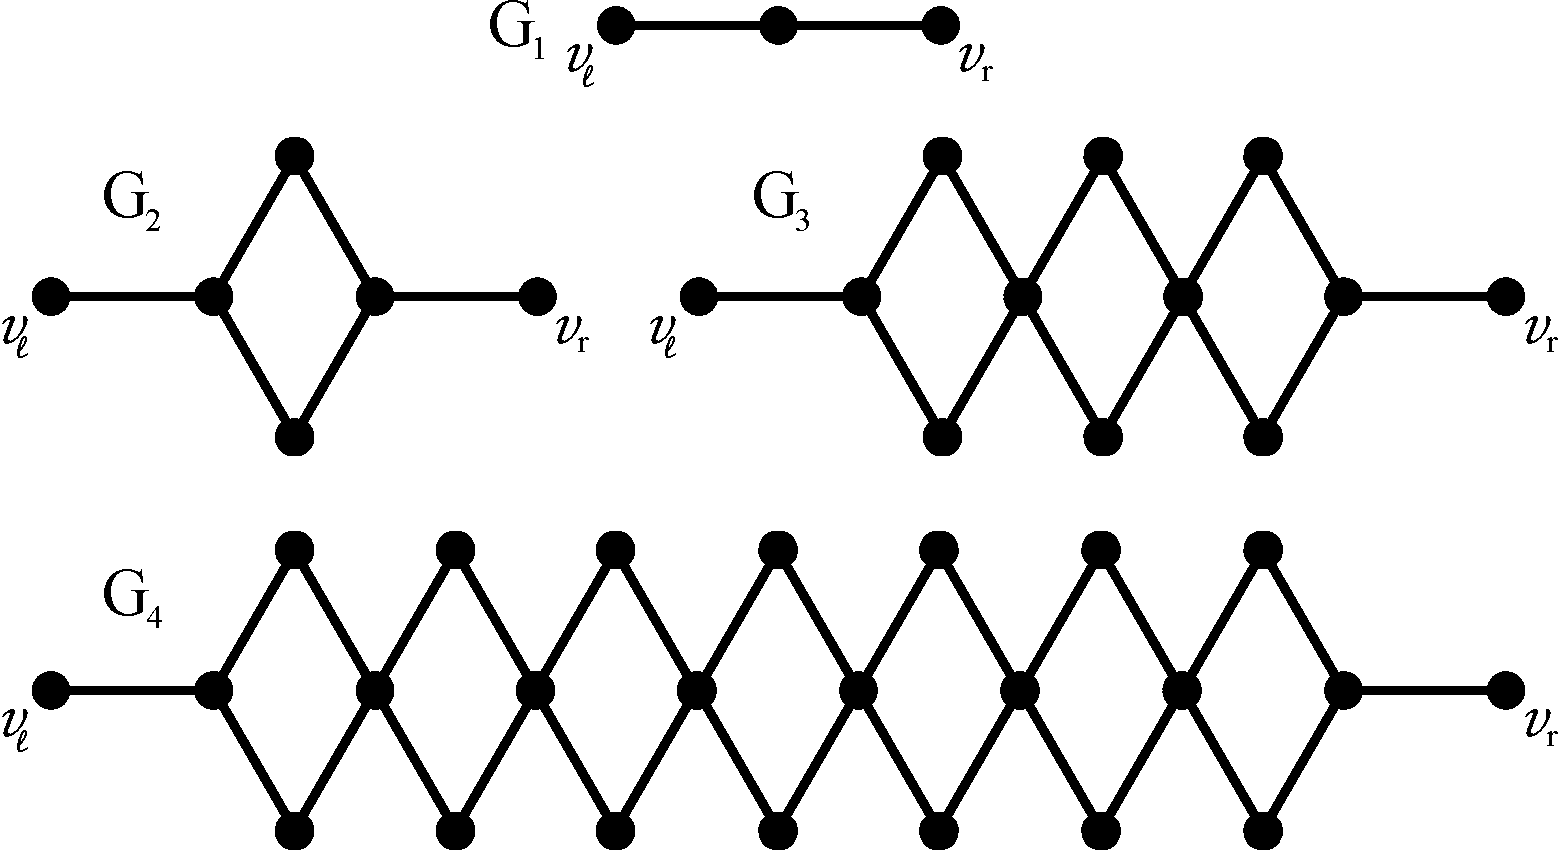
\includegraphics[scale=0.3]{imgs/concertina.pdf}
  \end{figure}
  \vfill
  \begin{theorem}
   The VC-dimension of $(\mathbb{S}_{G_i}, F)$ is $\lfloor\log_2\mathsf{VD}(G)
   -2\rfloor +1=i$
  \end{theorem}
  %\vfill
  %Proof Intuition: The middle vertices are internal to a lot of SPs
\end{frame}

%\begin{frame}
%  \frametitle{Is the Vertex-Diameter the right quantity?}
%  No! If $G$ undirected and for every connected pair of nodes there is a
%  unique SP, then the \emph{VC-dimension is at most 3}\\
%  \quad These graphs are not just trees!
%  \vfill
%  Proof: in such a graph, two SPs that meet and separate can not meet again\\
%  \quad (+ multiple case analysis)
%  \vfill
%  The bound ``3'' is tight. In the following graph we can shatter 3 paths
%  \begin{figure}[H]
%    \centering
%    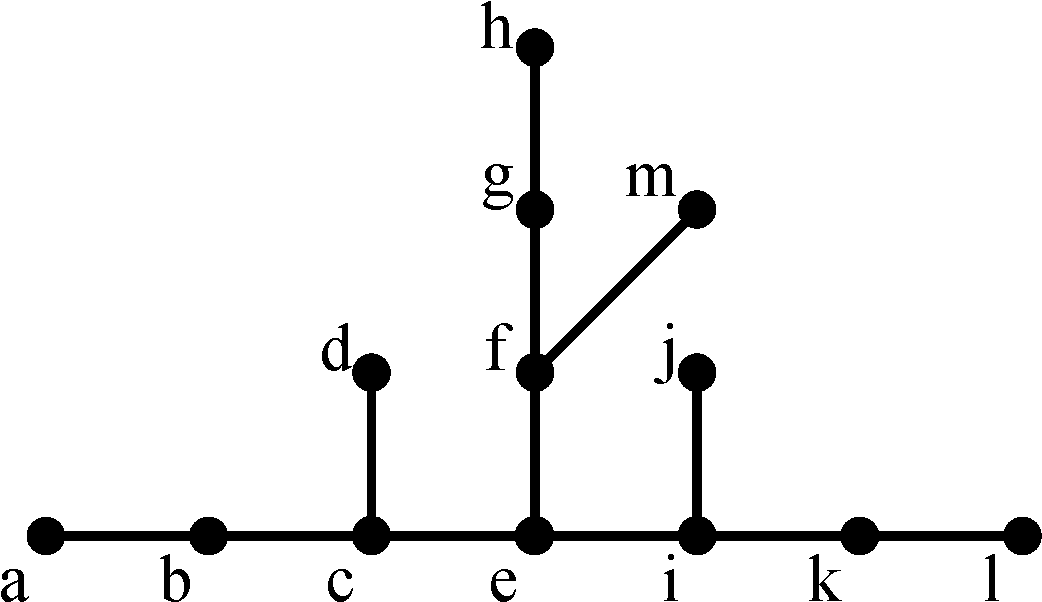
\includegraphics[scale=0.3]{imgs/uniqueshortestpathtight.pdf}
%  \end{figure}
%  \vfill
%  There is room for improvement using pseudodimension (we are working on that!)
%\end{frame}
%
%\begin{frame}
%  \frametitle{What about directed graphs?}
%  Does a similar result also hold for directed graphs with unique SP?\\
%  \quad  Not for the same constant $3$. We built a graph with unique SPs between
%  all connected nodes and we can shatter a set of $4$ SPs
%  \begin{figure}[H]
%    \centering
%    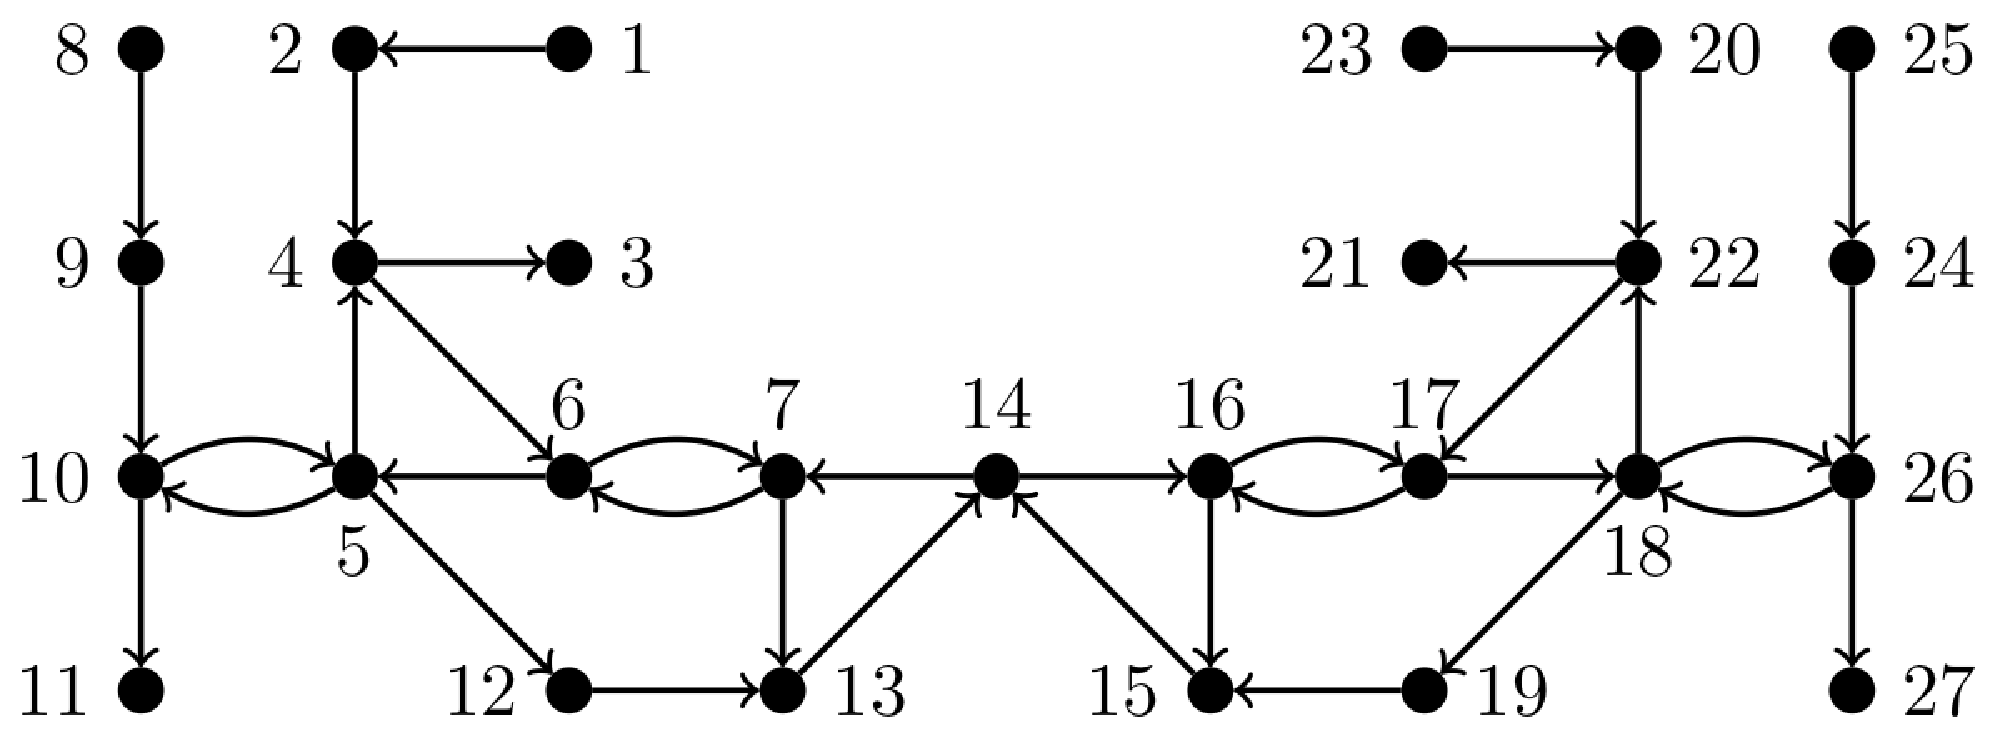
\includegraphics[scale=0.3]{imgs/uniquedirected.pdf}
%  \end{figure}
%  Yes, finding counterexamples is messy\ldots
%  \vfill
%  Does it hold for a different constant?\\
%  \quad We do not know! Maybe you can work on that?
%\end{frame}

\begin{frame}
  \frametitle{How well does the algorithm perform in practice?}
  It performs very well!
  \vfill
  We tested the algorithm on real graphs (SNAP) and on artificial
  Barabasi-Albert graphs, to evalue its accuracy, speed, and scalability
  \vfill
  Results: It blows away the exact algorithm and the union-bound-based
  sampling algorithm
\end{frame}

\begin{frame}
  \frametitle{How accurate is the algorithm?}
  In $O(10^3)$ runs of the algorithm on different graphs and with different
  parameters, we always had $|\tilde{\betw}(v)-\betw(v)|<\varepsilon$ for all
  nodes\\
  \quad Actually, on average $|\tilde{\betw}(v)-\betw(v)|<\varepsilon/8$
  \vfill
  \begin{figure}[H]
    \centering
    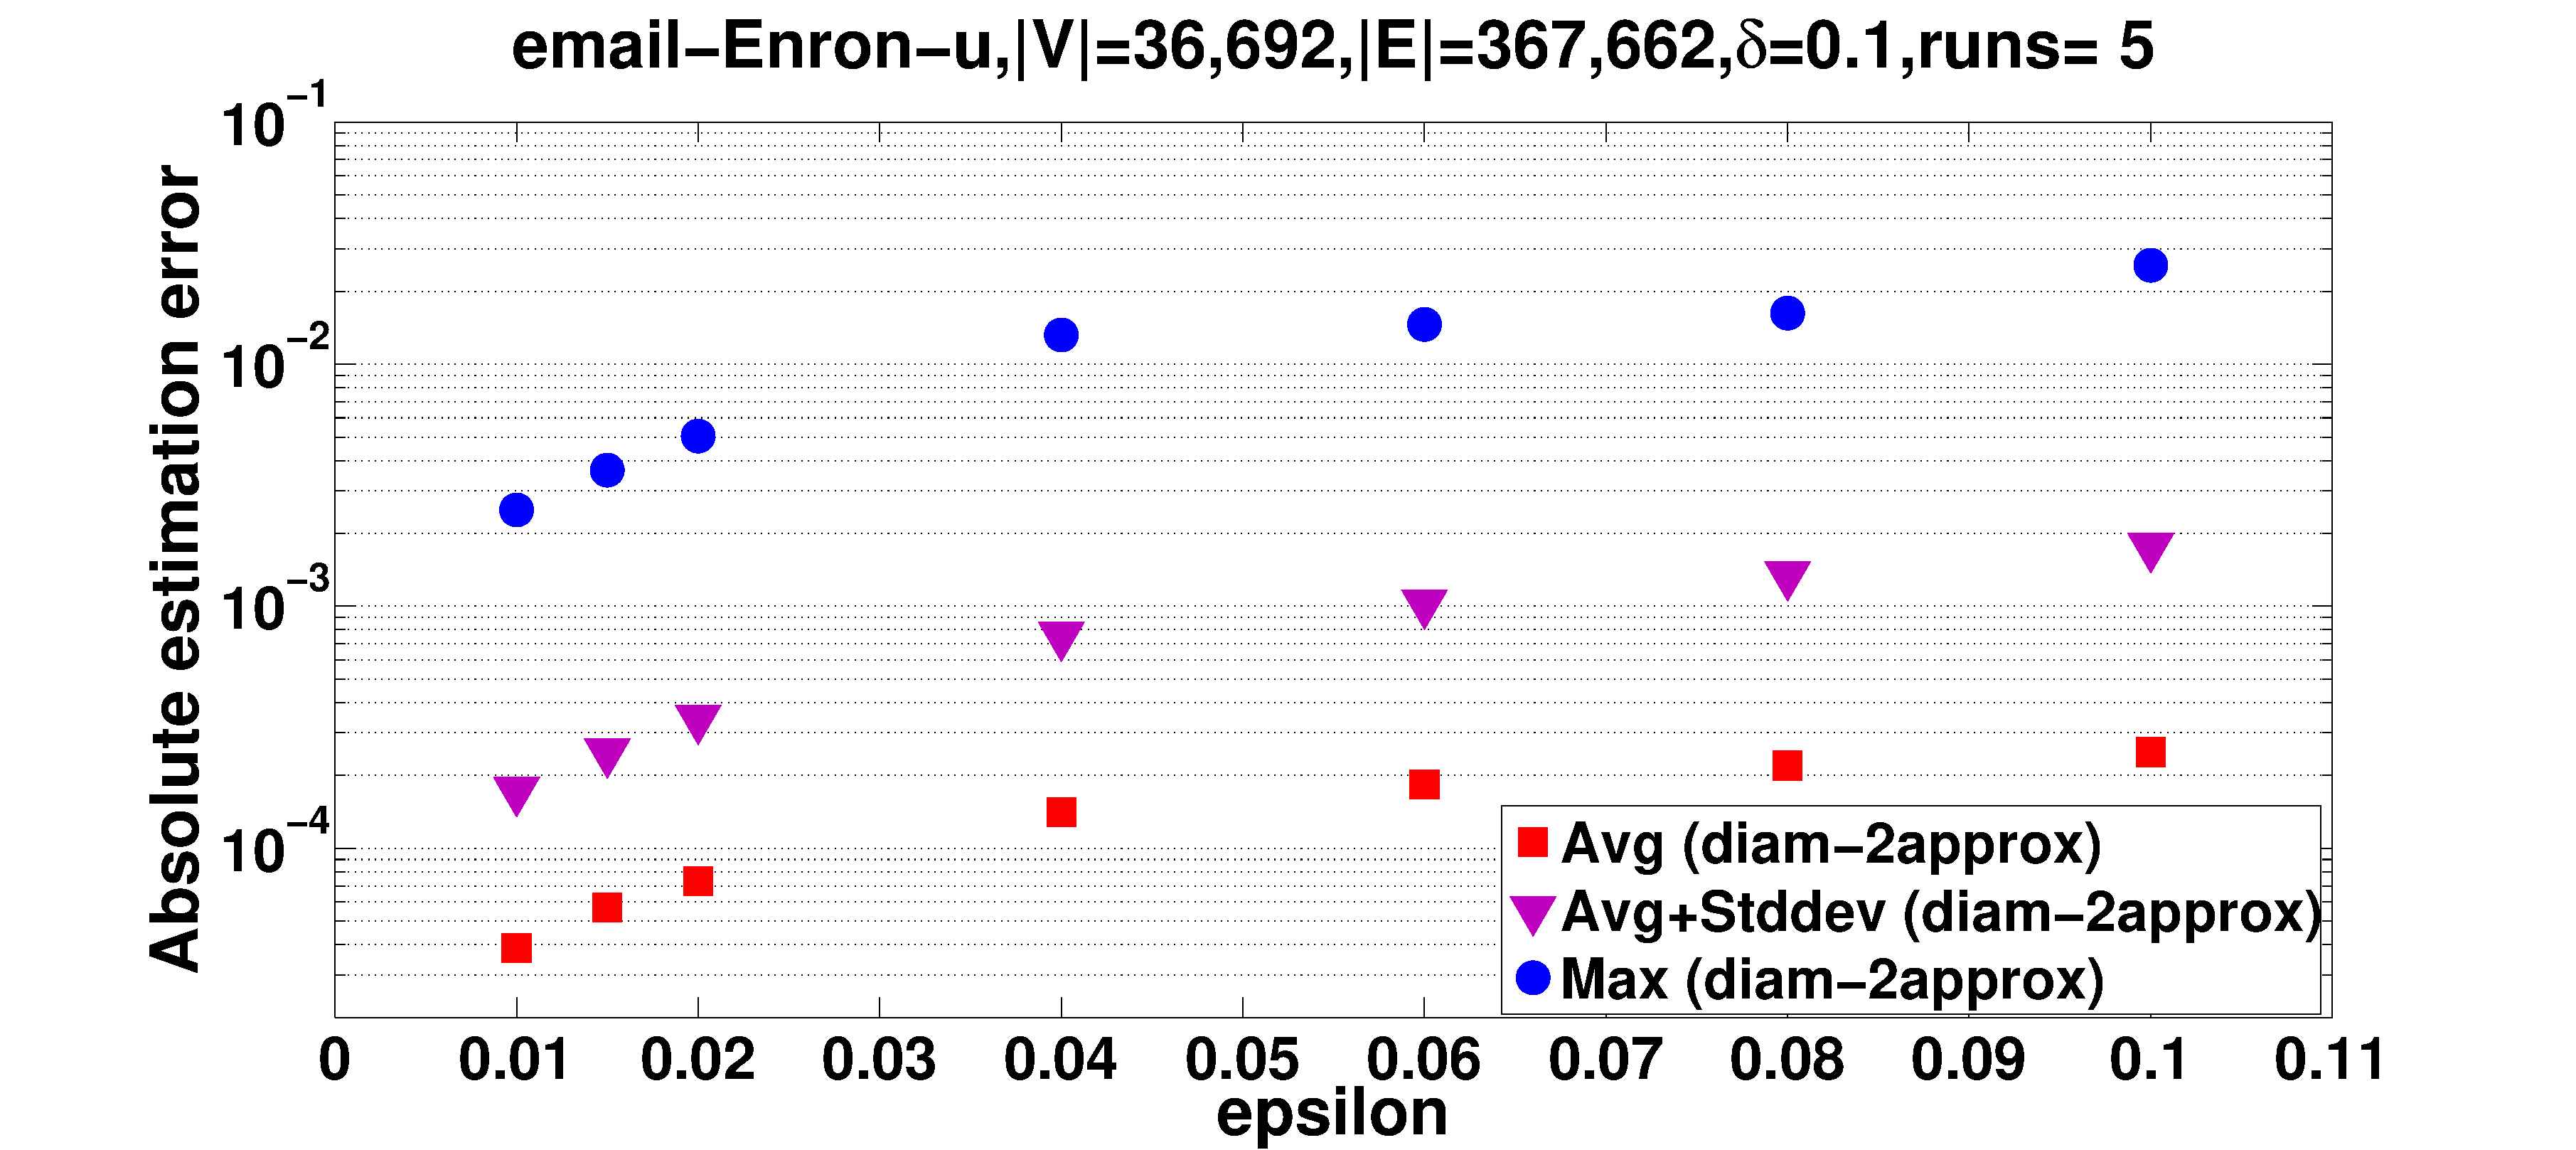
\includegraphics[width=\textwidth]{imgs/email-Enron-error.pdf}
  \end{figure}
\end{frame}

\begin{frame}
  \frametitle{How fast is the algorithm?}
  Approximately 8 times faster than the simple sampling algorithm
  \vfill
  Variable speedup w.r.t.~exact algorithm (200x -- 4x), depending on
  $\varepsilon$
  \vfill
  \begin{figure}[H]
    \centering
    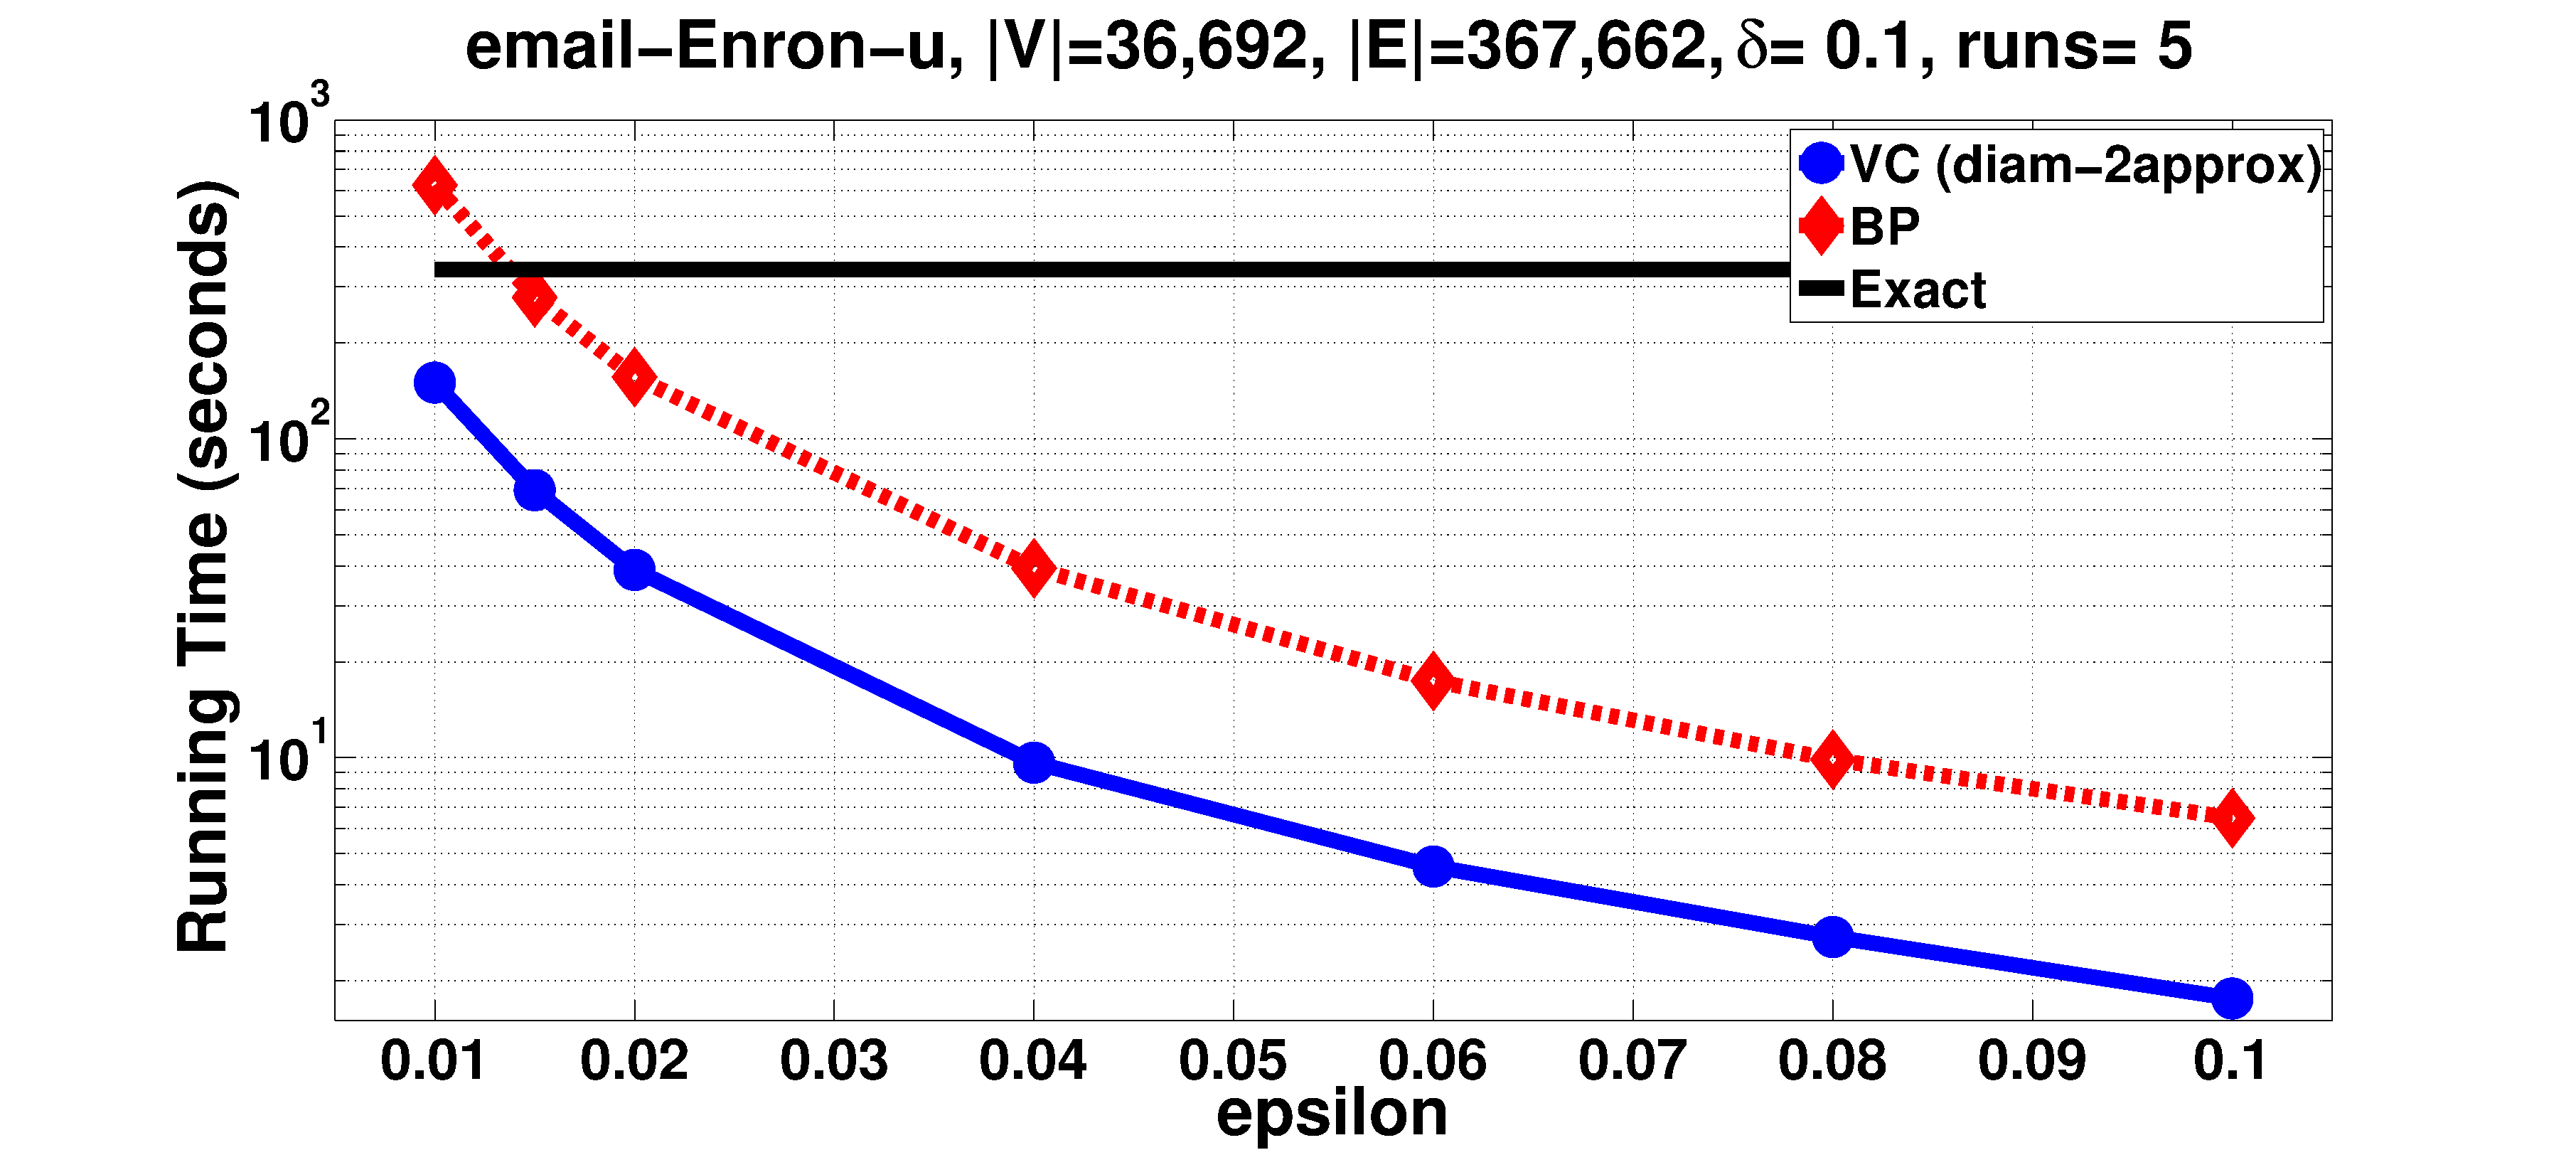
\includegraphics[width=\textwidth]{imgs/email-Enron-time.pdf}
  \end{figure}
\end{frame}

\begin{frame}
  \frametitle{How scalable is the algorithm?}
  Much more scalable than the simple sampling algorithm, because the sample
  size does not depend on $n$
  \vfill
  \begin{figure}[H]
    \centering
    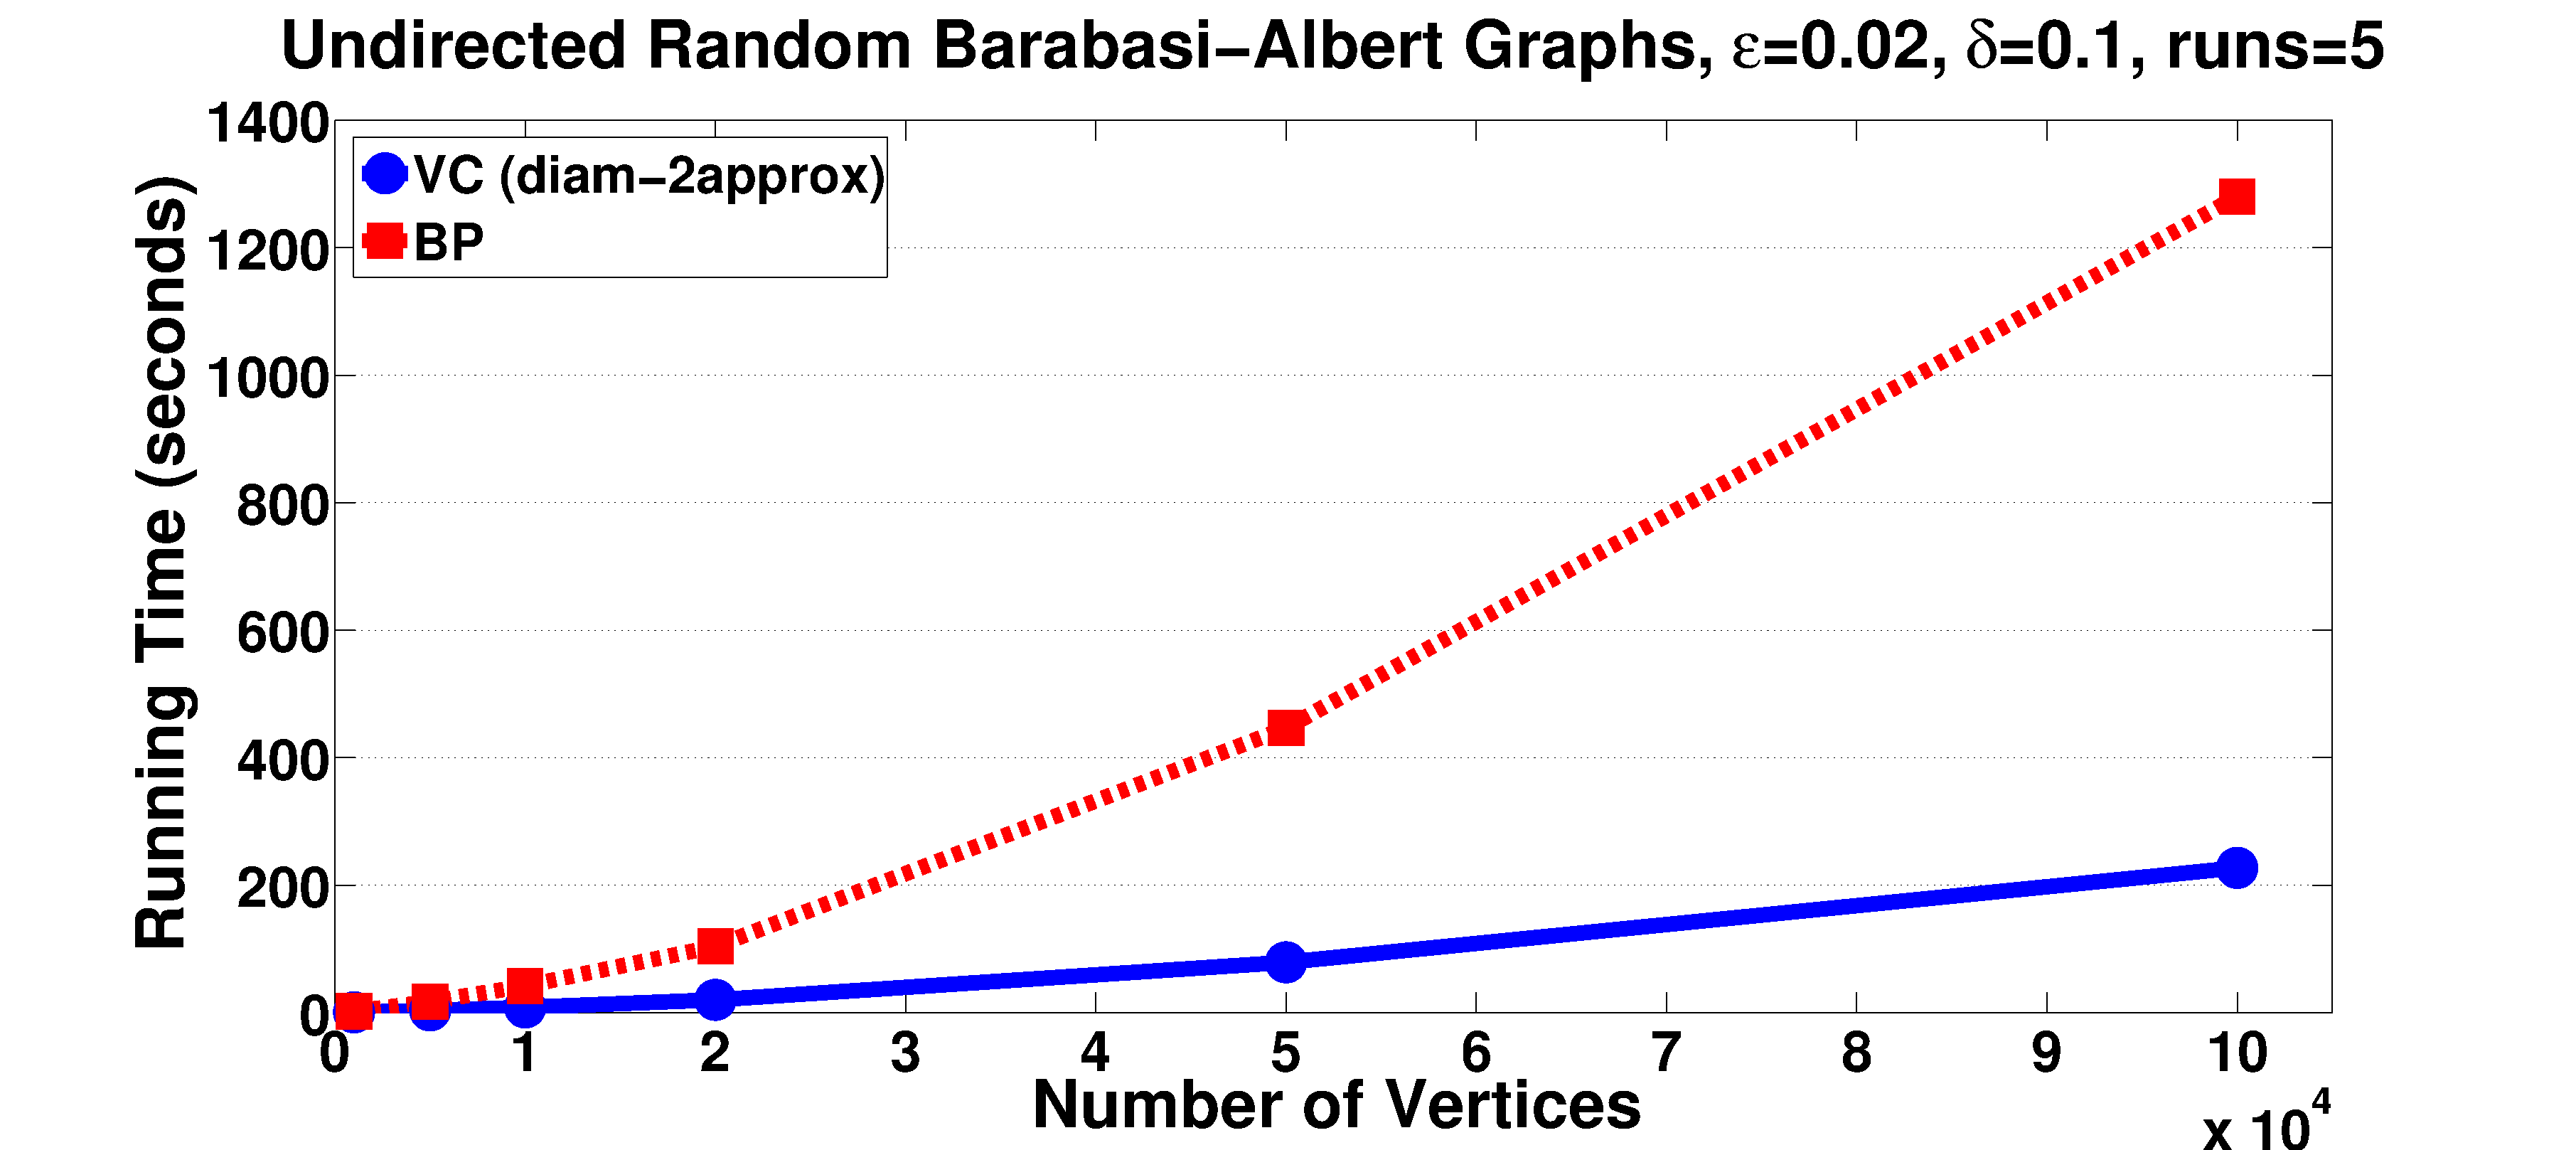
\includegraphics[width=\textwidth]{imgs/random-time.pdf}
  \end{figure}
\end{frame}

%\begin{frame}
%  \frametitle{Conclusions (Betweenness Centrality)}
%  \vfill
%  We showed a sampling algorithm for betweenness centrality approximation that
%  gives probabilistic guarantees on the quality of the approximation for all
%  the vertices
%  \vfill
%  The algorithm samples SPs according to a well-defined distribution, and
%  the analysis relies on VC-dimension, which is bounded by the Vertex Diameter,
%  a characteristic quantity of the graph that is small in real networks
%  \vfill
%  The use of VC-dimension makes the algorithm much faster and more scalable
%  than previous sampling approaches and than the exact algorithm
%\end{frame}

\begin{frame}
  \centering
  \vfill
  {\huge ABRA: Approximating Betweennes Centrality in Static and Dynamic
  Graphs with Rademacher Averages}
  \vfill
  {\large M.~Riondato, E.~Upfal}
  \vfill
  {\large arXiv (2016)}
  \vfill
\end{frame}

\begin{frame}
  \frametitle{Issues with RK approach}
  \begin{itemize}
    \item For each $s-t$ SP computation, we only \emph{use a single SP}
      \begin{itemize}
        \item a lot of wasted work!
      \end{itemize}
      \pause
    \item Must compute (upper bound to) the vertex-diameter before we can start
      sampling
      \begin{itemize}
        \item Exact computation cannot be done (would be equivalent to obtain
          exact betweenness)
        \item Approximate computation leads to larger-than-necessary sample size
      \end{itemize}
      \pause
  \end{itemize}
\end{frame}

\begin{frame}
  \frametitle{How to solve these issues}
  \begin{itemize}
    \item Design a sample scheme that uses \emph{all SPs} between a sampled pair
      of vertices
    \pause
    \item Use \emph{progressive sampling}, rather than static sampling
      \begin{itemize}
        \item Start from small sample size
        \item Check \emph{stopping condition} to verify whether we sampled
          enough to get a $(\varepsilon,\delta)$-approximation
        \item If yes, stop, otherwise keep sampling.
      \end{itemize}
  \end{itemize}
  \pause
  How to achieve this: using \emph{Rademacher averages} (VC-dimension on
  steroids)
\end{frame}

\begin{frame}
  \frametitle{Key ideas}
  \begin{itemize}
    \item When backtracking from $t$ to $s$, follow all SPs, not just one of
      them, and increase the estimation of all vertices found along the way: no
      wasted work;
    \pause
    \item  The stopping condition depends on:
      \begin{itemize}
        \item the \emph{richness} of the vectors representing the current
          estimates of the betweenness of all vertices
        \pause
        \item the current sample size
        \pause
      \item Formulas like this:
        \[
          \frac{1}{1-\alpha}\min_{s\in\mathbb{R}^+}\frac{1}{s}\ln\sum_{\mathbf{v}\in\mathcal{V}_\Sam}\mathrm{exp}(s^2\|\mathbf{v}\|^2/(2\ell^2))
          +\frac{\ln\frac{2}{\delta}}{2\ell\alpha(1-\alpha)}+\sqrt{\frac{\ln{2/\delta}}{2\ell}}
        \]
      \end{itemize}
    \pause
    \item But it works!
  \end{itemize}
\end{frame}

\begin{frame}
  \frametitle{Experiments}
  \begin{figure}
    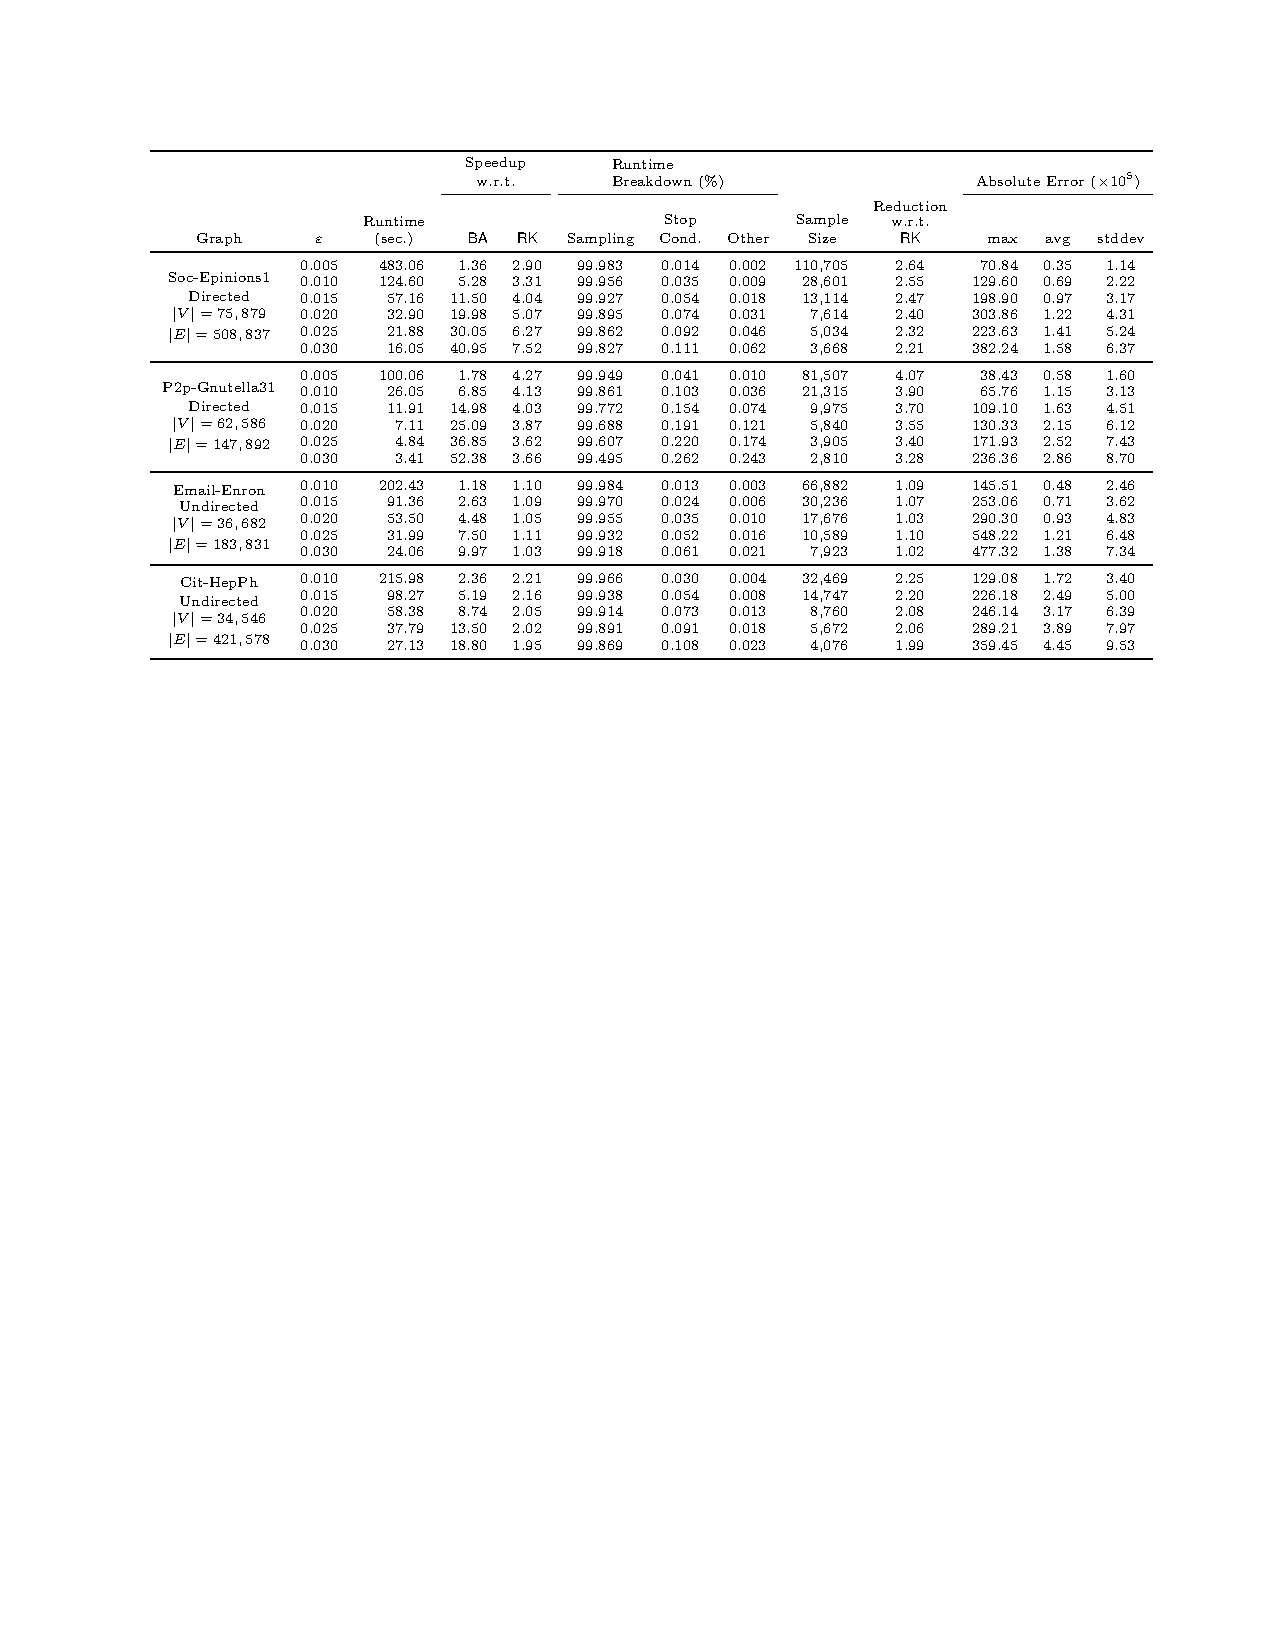
\includegraphics[width=\textwidth]{imgs/RiondatoU-table.pdf}
  \end{figure}
  \begin{itemize}
    \item Smaller sample sizes than RK
    \item Much faster (not just because using smaller sample, also because no
      need to compute the vertex-diameter)
    \item Very accurate
  \end{itemize}
\end{frame}

\begin{frame}
  \frametitle{Experiments}
  \begin{figure}
    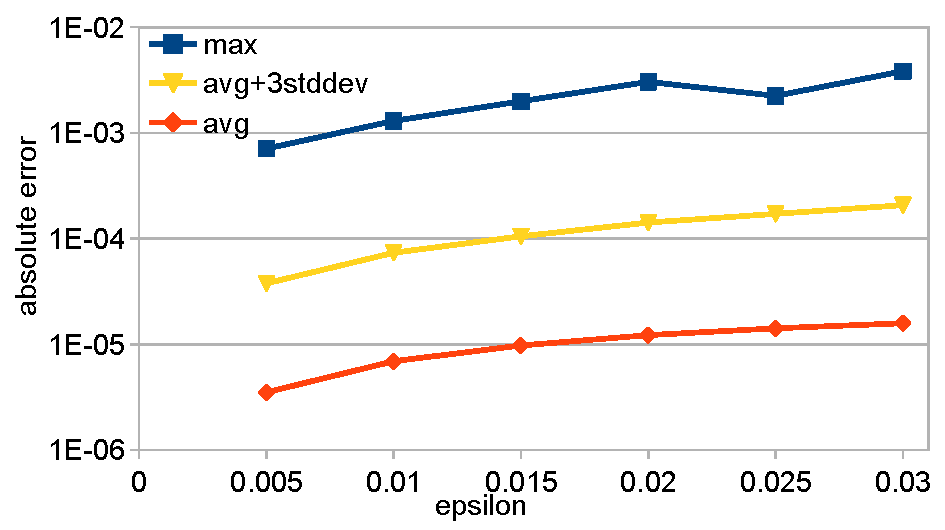
\includegraphics[width=\textwidth]{imgs/epinions-error.pdf}
  \end{figure}
  \begin{itemize}
    \item More than 10x more accurate than guaranteed, on average;
    \item More than 100x more accurate than guaranteed, in the best case;
    \item Close to the guarantee in the worst case: this is good.
  \end{itemize}
\end{frame}

\subsection{Approximation Algorithms for Dynamic Graphs}

\begin{frame}
  \centering
  \vfill
  {\huge Fully-Dynamic Approximation of Betweenness Centrality}
  \vfill
  {\Large E.~Bergamini, H.~Meyerhenke}
  \vfill
  {\large ESA: European Symposium on Algorithms (2015)}
  \vfill
\end{frame}

\begin{frame}
  \frametitle{Key ideas}
  This algorithm builds on:
  \begin{itemize}
    \item the RK sampling-based approximation algorithm;
    \item existing algorithms to update the SP DAG after an insertion/removal of
      a batch of edges;
  \end{itemize}
  \pause
  \vfill
  It keeps track of potential modifications to the vertex diameter to
  understand whether to increase the sample size;
  \pause
  \vfill
  \begin{theorem}
    After each batch update, the output is an
    $(\varepsilon,\delta)$-approximation.
  \end{theorem}
\end{frame}

\begin{frame}
  \frametitle{Updating the DAGs}
  \begin{itemize}
    \item Never change the set of sampled pairs of vertices, unless a sample was removed
      or more samples are needed
    \item What can change is which SP is sampled: if an edge is added, the path
      we sampled before may no longer be a SP.
      \pause
    \item In any case, must save \emph{all the SP DAGs} between the sampled
      pair of nodes
      \pause
    \item Requires a lot of memory, but is needed in order to be able to update
      the estimation after the batch update
    \item The update computation builds on existing algorithms
  \end{itemize}
\end{frame}

\begin{frame}
  \frametitle{Keeping track of the vertex diameter}
  \begin{itemize}
    \item An edge is removed: the VD may decrease, but no need to change the
      sample size;
    \pause
    \item An edge is added between two existing vertices in the same connected
      component: no change in the VD, hence no change in sample size
    \pause
    \item An edge is added between two existing vertices in two different
      connected components: the VD may have changed, recomputation is necessary
    \pause
    \item An edge is added between an existing vertex and a new vertex: the VD
      may have increased by one, recomputation is necessary (the model used in
      this paper does not actually consider the insertion and removal of
      vertices)
  \end{itemize}
  \pause
  Relying on the vertex diameter is not a great idea, that's why we developed
  ABRA, the Rademacher Averages-based algorithm.
\end{frame}

\begin{frame}
  \frametitle{Experiments}
  \begin{figure}
    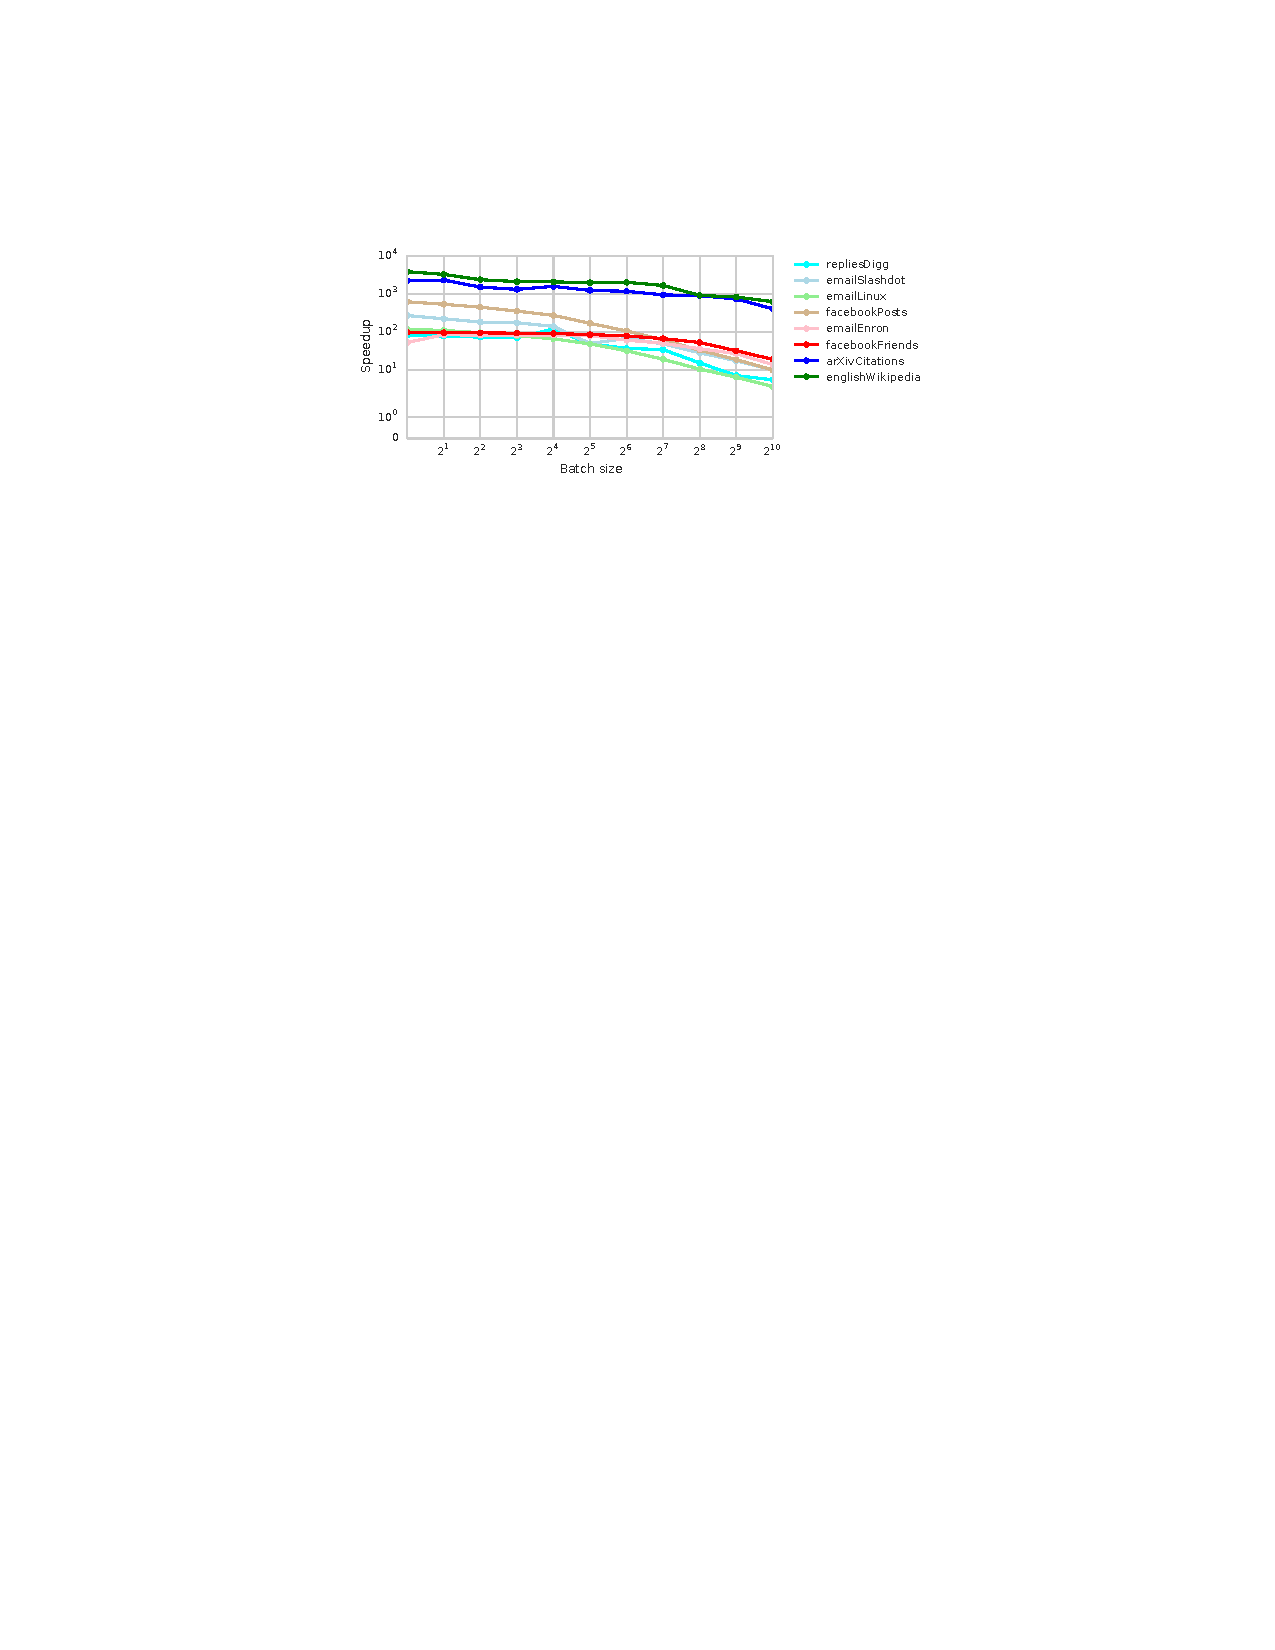
\includegraphics[width=\textwidth]{imgs/Bergamini-speedup.pdf}
  \end{figure}
  Speedup over RK
\end{frame}

\begin{frame}
  \centering
  \vfill
  {\huge Fully Dynamic Betweenness Centrality Maintenance on Massive
  Networks}
  \vfill
  {\Large T.~Hayashi, T.~Akiba, Y.~Yoshida}
  \vfill
  {\large VLDB: Very Large Databases (2016)}
  \vfill
\end{frame}

\begin{frame}
  \frametitle{Key ideas}
  \begin{itemize}
    \item Still a sampling-based approximation algorithm, but samples pair of
      vertices;
    \item This similar to RU16, but analysis use the union bound, so
      $O(\varepsilon^{-2}\log n)$ samples, which is a lot;
    \item Presents a new data structure called \emph{hypergraph sketch} to keep
      track of the SP DAGS.
      \pause
       \item An additional data structure, called the Two-ball Index, allows to
      identify the parts of hypergraph sketches that require updates
  \end{itemize}
\end{frame}

\begin{frame}
  \frametitle{The Hypergraph Sketch}
  (effectively a hypergraph)
  \begin{itemize}
    \item For each sampled pair $(s,t)$ of vertices, an \emph{hyperedge} is
      added to the hypergraph:
      \[
        e_{st}=\{(v,\sigma_{sv}, \sigma_{v,t}) : v \text{ is on a SP from $s$ to
        $t$}\}
      \]
      \pause
    \item The estimations $\tbetw(v)$ can be obtained from the sketch;
      \pause
    \item Handling insertion and removal of edges is straightforward, but must
      be done efficiently
    \item Handling insertion and removal of nodes requires to change the set of
      sampled pair of vertices, i.e., to potentially remove a hyperedge and
      insert another one;
  \end{itemize}
\end{frame}

\begin{frame}
  \frametitle{Vertex Operations}
  \begin{figure}
    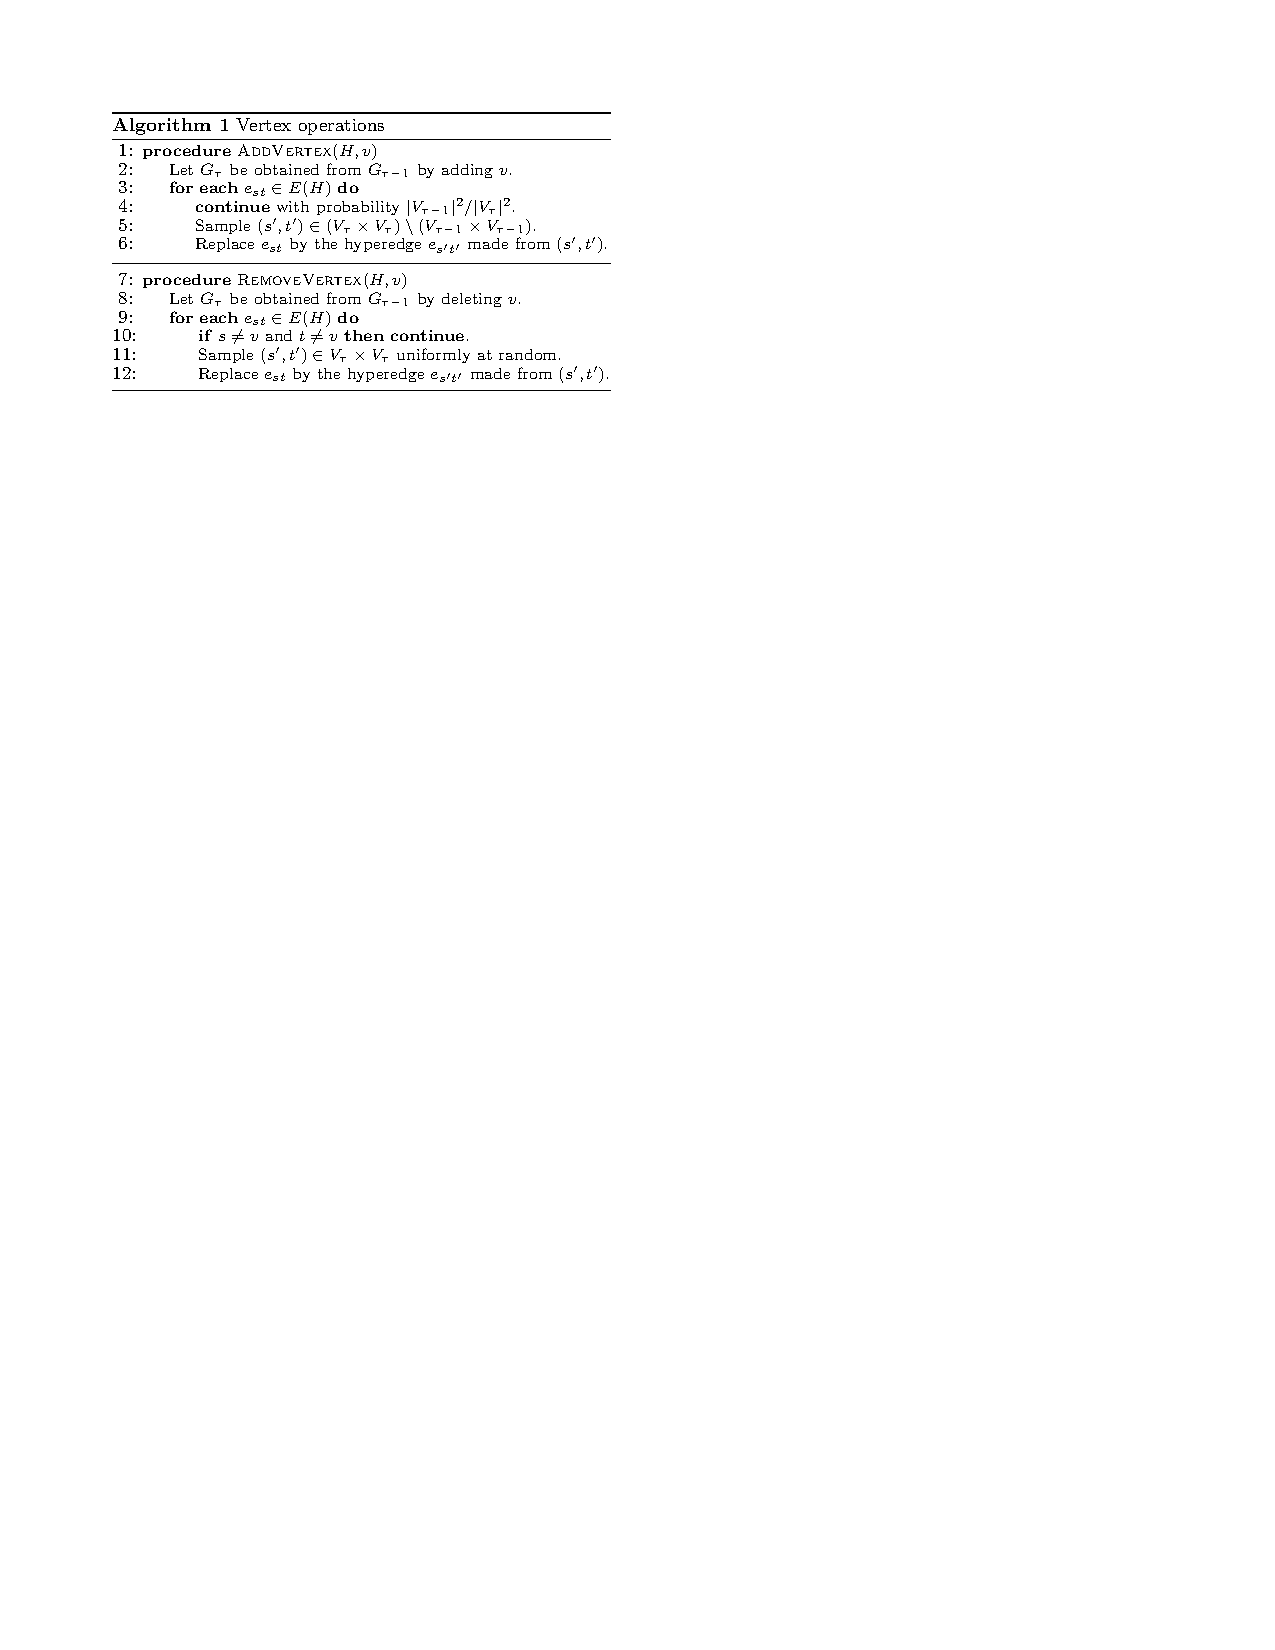
\includegraphics[width=\textwidth]{imgs/Ayashi-pseudocode.pdf}
  \end{figure}
\end{frame}

\begin{frame}
  \frametitle{The Two-Ball Index}
  \begin{itemize}
    \item For each sampled pair $(s,t)$, maintain a triplet $(\Delta_{st},
      \beta^+, \beta^-)$, where
      \begin{itemize}
        \item $\Delta_{st}=\{d(s,v), v  \text{ is on a SP from $s$ to
        $t$}\}$
      \item The ball $\beta^+$ is the set of vertices at distance less than some $d_s$
        from $s$, with their distances
      \item The ball $\beta^+$ is the set of vertices at distance less than some $d_t$
        from $t$, with their distances
    \end{itemize}
  \item The radiuses of the balls are such that they do not touch and are small.
  \item The triplets can be built with a bidirectional SP computation
    from $s$ to $t$
  \end{itemize}
\end{frame}

\begin{frame}
  \frametitle{Update Mechanism (for insertion)}
  \begin{figure}
    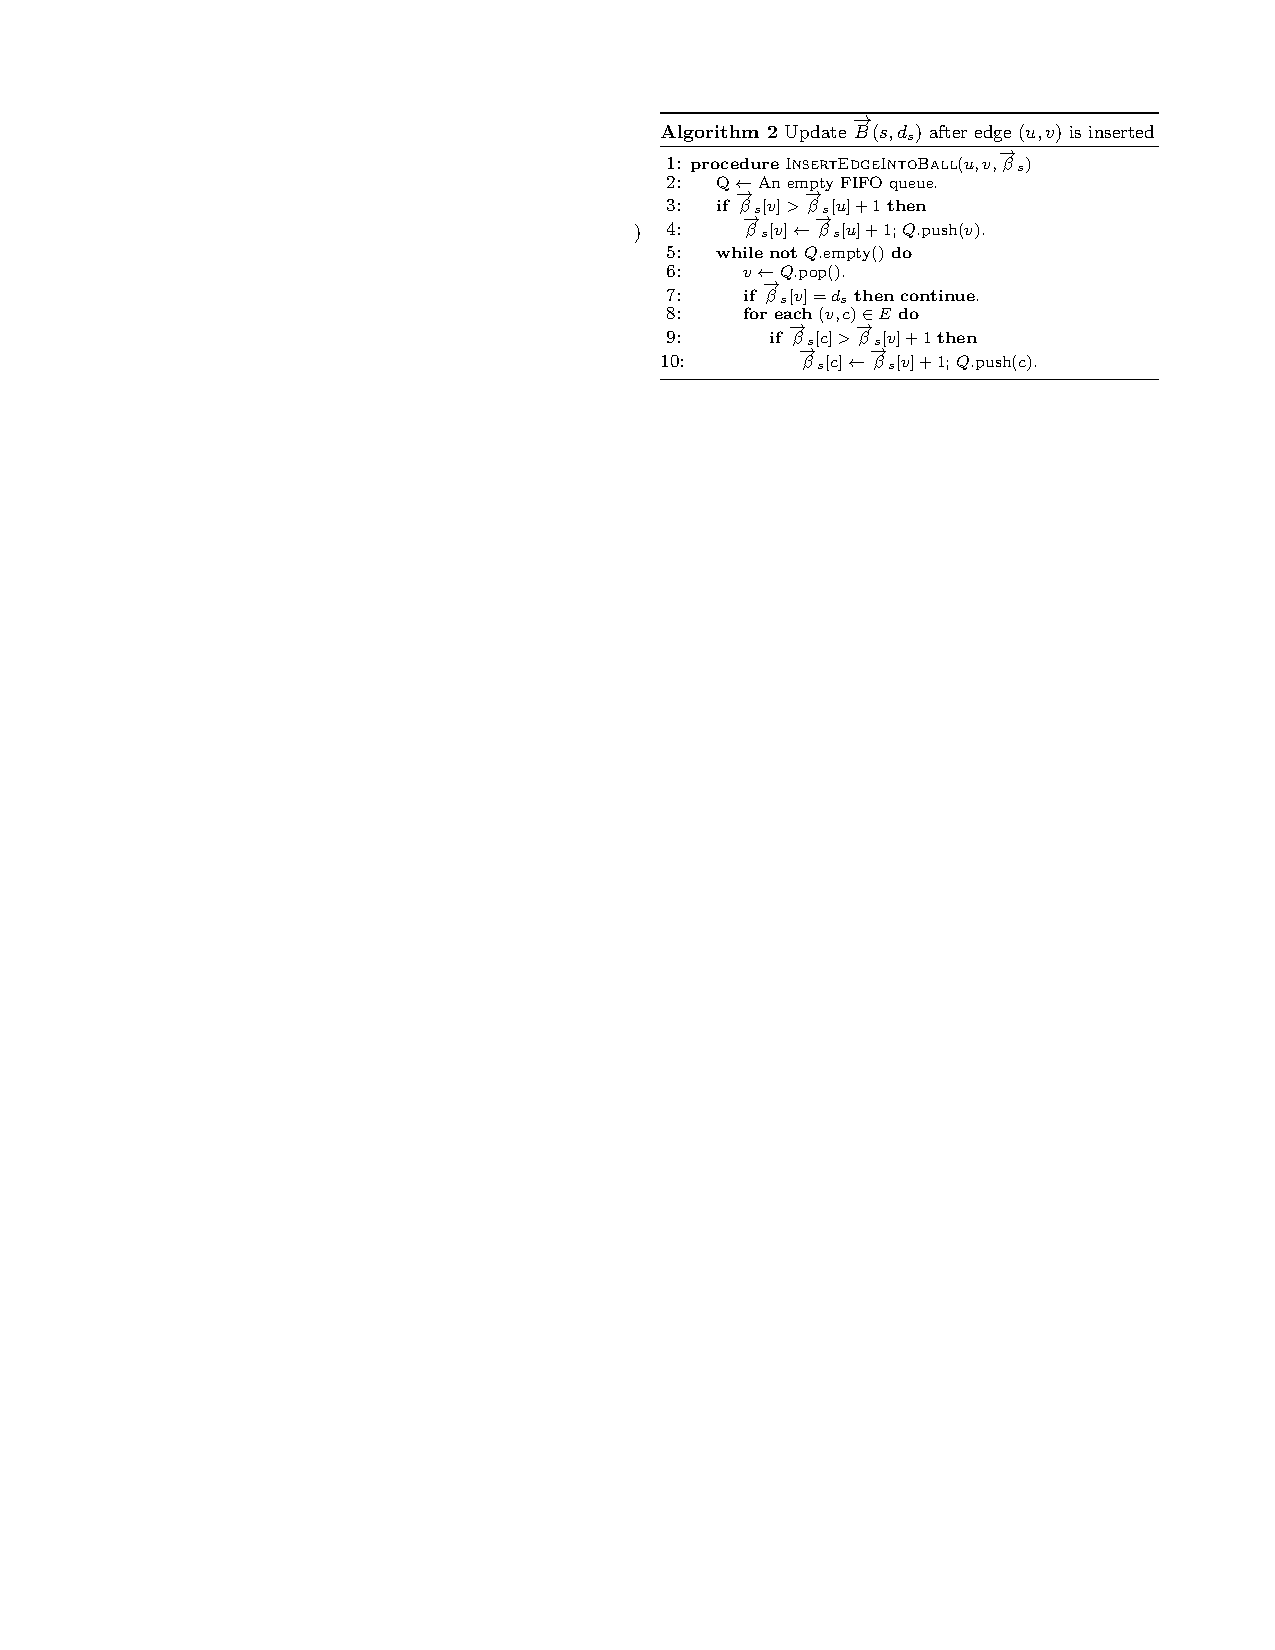
\includegraphics[width=\textwidth]{imgs/Ayashi-pseudocodeupdate.pdf}
  \end{figure}
  \pause
  (much more complex for deletion)
\end{frame}

\begin{frame}
  \frametitle{Experiments}
  \begin{figure}
    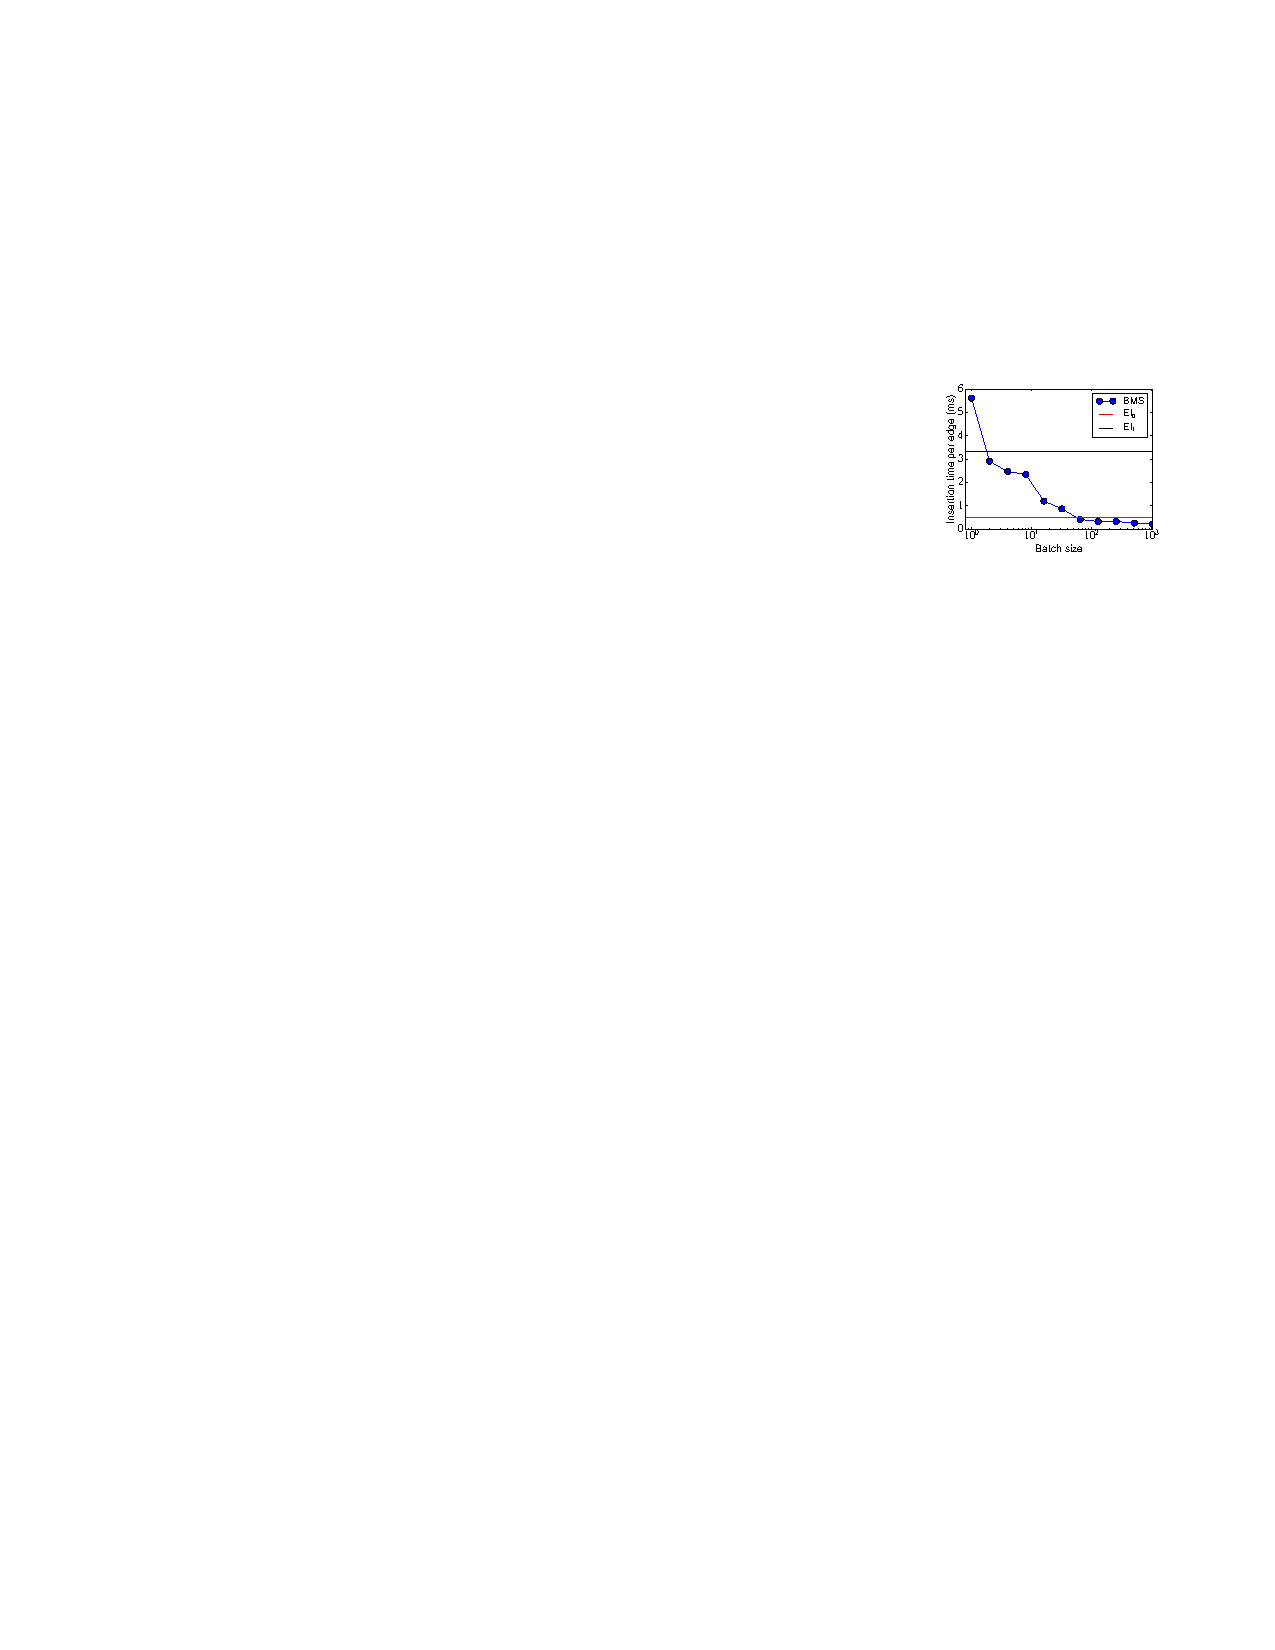
\includegraphics[width=0.7\textwidth]{imgs/Ayashi-expers.pdf}
  \end{figure}
\end{frame}

\begin{frame}
  \frametitle{Summary on approximation algorithms for betweenness}
  \begin{itemize}
    \item Sampling Rules Everything Around Me;
      \pause
    \item Work on pushing down the amount of needed sampling is important;
      \pause
    \item Progressive sampling frees us from many worries, but it is
      challenging;
      \pause
    \item  Fast and memory efficient data structures are needed to be able to
      update the estimations fast in dynamic graphs, where approximation is
      most useful;
      \pause
    \item Developing hybrid estimators?
  \end{itemize}
\end{frame}
